%%!TEX root = diss.tex

\chapter{Collisional Langevin model of bedload sediment velocity distributions}
\label{ch:langevin}
\section{Introduction}

\DIFdelbegin \DIFdel{Bed load }\DIFdelend \DIFaddbegin \DIFadd{Bedload }\DIFaddend transport rates show wide and frequent fluctuations which originate from coupling between the fluid and granular phases.
Owing to these fluctuations, measured transport rates often show slow convergence through time \citep{Dhont2018,Turowski2010}, and predicted rates can deviate from measured values by several orders of magnitude \citep{Recking2012,Martin2003}.
These challenges limit numerous ecological and engineering applications that rely on sediment transport predictions \citep{Gaeuman2017,Malmon2005}.
\DIFaddbegin 

\DIFaddend In recent decades, stochastic formulations of the \DIFdelbegin \DIFdel{bed load }\DIFdelend \DIFaddbegin \DIFadd{bedload }\DIFaddend flux have become increasingly popular for their potential to predict the mean transport rates required by applications while also predicting the magnitude of transport fluctuations and quantifying the dependence of measurements on the observation scale (\DIFdelbegin \DIFdel{secs. \ref{sec:birthdeath} -}\DIFdelend \DIFaddbegin \DIFadd{Secs. \ref{sec:birthdeath} and }\DIFaddend \ref{sec:renewal}).
Recent indications that sediment transport fluctuations might explain longstanding open problems in alluvial channel stability, such as channel width maintenance \citep{Abramian2019,Abramian2020} and bedform initiation \citep{Jerolmack2005,Bohorquez2016} provide additional motivation to develop these stochastic approaches.
One subset of stochastic methods expresses downstream transport rates as a sum over the instantaneous streamwise velocities of all particles in motion within a control volume (\DIFdelbegin \DIFdel{sec}\DIFdelend \DIFaddbegin \DIFadd{Sec}\DIFaddend . \ref{sec:birthdeath}).
This formulation requires the instantaneous velocity distributions of sediment particles \DIFdelbegin \DIFdel{\mbox{%DIFAUXCMD
\citep{Lajeunesse2010}}\hspace{0pt}%DIFAUXCMD
, although }\DIFdelend \DIFaddbegin \DIFadd{\mbox{%DIFAUXCMD
\citep[e.g.][]{Ancey2020a}}\hspace{0pt}%DIFAUXCMD
, yet our }\DIFaddend understanding of these distributions remains limited.
There is as of yet no consensus on the shape of the bedload velocity distribution, and although the models described in \DIFdelbegin \DIFdel{section \ref{sec:langevin} of the introduction have described }\DIFdelend \DIFaddbegin \DIFadd{Sec. \ref{sec:langevin} describe }\DIFaddend some extreme end-member distributions \citep[e.g.][]{Fan2014,Ancey2014}, no models have been developed that describe \DIFdelbegin \DIFdel{the full range of experimental observations }\DIFdelend \DIFaddbegin \DIFadd{all experimental observations reported to date }\DIFaddend \citep{Lajeunesse2010,Fathel2015,Heyman2016,Liu2019,Houssais2012}.
In this chapter, I develop a stochastic model of particle velocities which addresses this shortcoming.

High-speed video experiments have measured different streamwise particle velocity distributions without indicating why one distribution or another appears in a given set of hydraulic and sedimentary conditions.
One set of studies has shown exponential particle velocity distributions \citep{Charru2004,Lajeunesse2010,Roseberry2012,Seizilles2014,Fathel2015,Fathel2016}.
These experiments involve uniformly-sized small sands or glass beads (\DIFdelbegin \DIFdel{$~0.05-2$}\DIFdelend \DIFaddbegin \DIFadd{$0.05-2$}\DIFaddend mm) in turbulent and subcritical flows, but not always; the experiments of \citet{Lajeunesse2010} were \DIFaddbegin \DIFadd{turbulent and }\DIFaddend supercritical, while the experiments of \citet{Charru2004} and \citet{Seizilles2014} were \DIFdelbegin \DIFdel{viscous}\DIFdelend \DIFaddbegin \DIFadd{laminar and (likely) subcritical}\DIFaddend .
A second set of studies \DIFdelbegin \DIFdel{have shown }\DIFdelend \DIFaddbegin \DIFadd{show }\DIFaddend Gaussian particle velocity distributions \citep{Ancey2014,Heyman2016,Martin2012}. In these experiments, particles are typically larger ($2-8$mm) uniformly-sized gravels or glass beads, and flows are generally turbulent and \DIFdelbegin \DIFdel{super-critical}\DIFdelend \DIFaddbegin \DIFadd{supercritical}\DIFaddend .
Other experiments display velocity distributions that are intermediate between exponential and Gaussian \DIFdelbegin \DIFdel{extremes }\DIFdelend that appear visually more like a Gamma distribution \citep{Houssais2012, Liu2019}.
\DIFdelbegin \DIFdel{The \mbox{%DIFAUXCMD
\citet{Houssais2012} }\hspace{0pt}%DIFAUXCMD
experiments involved a binomal }\DIFdelend \DIFaddbegin \DIFadd{\mbox{%DIFAUXCMD
\citet{Houssais2012} }\hspace{0pt}%DIFAUXCMD
used a bimodal }\DIFaddend distribution of glass beads with diameters $0.7$mm and $2.2$mm in turbulent and supercritical flow conditions, while \DIFdelbegin \DIFdel{the \mbox{%DIFAUXCMD
\citet{Liu2019} }\hspace{0pt}%DIFAUXCMD
experiments }\DIFdelend \DIFaddbegin \DIFadd{\mbox{%DIFAUXCMD
\citet{Liu2019} }\hspace{0pt}%DIFAUXCMD
}\DIFaddend used sand having median diameter $1.1$mm \DIFdelbegin \DIFdel{. Flows were again }\DIFdelend \DIFaddbegin \DIFadd{in }\DIFaddend turbulent and subcritical \DIFaddbegin \DIFadd{flow}\DIFaddend .
From this experimental record, the velocity distribution shape apparently does not consistently relate to \DIFdelbegin \DIFdel{super or sub-critical flow conditions , whether sediment grains are natural (sand, gravel ) or synthetic (}\DIFdelend \DIFaddbegin \DIFadd{the flow conditions (turbulent/laminar or super/subcritical) or sediment properties (natural sand/gravel or }\DIFaddend glass beads)\DIFdelbegin \DIFdel{, or whether the flow is laminar or turbulent}\DIFdelend .
However there is a loose trend within the particle size.
Smaller particles tend to show more exponential-like distributions \citep[e.g.][]{Fathel2015}, while larger ones show Gaussian distributions \citep[e.g.][]{Heyman2016}. This summary suggests that \DIFdelbegin \DIFdel{the shape of streamwise bed load }\DIFdelend \DIFaddbegin \DIFadd{bedload }\DIFaddend velocity distribution could be controlled by the particle size.

Existing models of streamwise \DIFdelbegin \DIFdel{bed load }\DIFdelend \DIFaddbegin \DIFadd{bedload }\DIFaddend velocities can be divided into computational and stochastic physics categories.
Computational models numerically integrate some approximate coupled dynamics for individual grains and the fluid, generally \DIFdelbegin \DIFdel{modelling }\DIFdelend \DIFaddbegin \DIFadd{modeling }\DIFaddend particles as spheres interacting through repulsive forces \DIFdelbegin \DIFdel{, and the flow using direct simulation of }\DIFdelend \DIFaddbegin \DIFadd{and numerically integrating }\DIFaddend the Navier-Stokes equations \DIFdelbegin \DIFdel{or some related approximation (such as large eddy simulation or the St-Venant equations) }\DIFdelend \DIFaddbegin \DIFadd{(or some approximation of them) to describe the flow forces on grains}\DIFaddend .
When streamwise particle velocities have been analyzed in such simulations, they show exponential tails \citep{Gonzalez2017,Furbish2013} that agree with one subset of the experimental data.

\DIFdelbegin \DIFdel{Several stochastic }\DIFdelend \DIFaddbegin \DIFadd{Stochastic }\DIFaddend models have incorporated fluctuating driving and resisting terms into \DIFdelbegin \DIFdel{the Newtonian dynamics }\DIFdelend \DIFaddbegin \DIFadd{Newtonian equations }\DIFaddend of individual grains to develop Langevin-like descriptions of \DIFdelbegin \DIFdel{bed load }\DIFdelend \DIFaddbegin \DIFadd{bedload }\DIFaddend particle motions (\DIFdelbegin \DIFdel{sec}\DIFdelend \DIFaddbegin \DIFadd{Sec}\DIFaddend . \ref{sec:langevin}). \citet{Fan2014} represented turbulent drag as Gaussian white noise and included a static Coulomb friction term to model particle-bed collisions, while \citet{Ancey2014} applied an Ornstein-Uhlenbeck process which combines the fluid and driving forces \DIFdelbegin \DIFdel{were lumped into a }\DIFdelend \DIFaddbegin \DIFadd{into a simplified }\DIFaddend velocity-dependent force, \DIFdelbegin \DIFdel{while }\DIFdelend \DIFaddbegin \DIFadd{again modeling fluctuations with }\DIFaddend Gaussian white noise\DIFdelbegin \DIFdel{represents fluctuations}\DIFdelend .
Each of these models derives one end-member distribution from among the range of distributions reported in experiments.
A physical description for the full range of experimentally-observed bedload velocity distributions remains an elusive target.

In this chapter I explore the possibility that the \DIFdelbegin \DIFdel{shape of the }\DIFdelend particle velocity distribution is controlled by momentum dissipation \DIFdelbegin \DIFdel{during }\DIFdelend \DIFaddbegin \DIFadd{from }\DIFaddend particle-bed collisions \DIFaddbegin \DIFadd{by incorporating ideas from the physics of granular media.
A major paradigm in granular dynamics is to describe particles as a continuum or "granular liquid" having an effective rheology \mbox{%DIFAUXCMD
\citep[e.g.][]{Jenkins1998,Andreotti2013}}\hspace{0pt}%DIFAUXCMD
, but as discussed in Ch. \ref{ch:Introduction} such a continuum assumption is unlikely to be satisfied for weak bedload transport conditions. 
}

\DIFadd{Instead,articles in these conditions are better characterized as a rarefied granular gas \mbox{%DIFAUXCMD
\citep[e.g.][]{Furbish2021}}\hspace{0pt}%DIFAUXCMD
}\DIFaddend . 
In the theory of \DIFaddbegin \DIFadd{rarefied }\DIFaddend granular gases, dissipative collisions are known to cause departures toward an exponential velocity distribution from the ideal Gaussian form expected from perfectly elastic collisions \citep{Brilliantov2004}.
Gas theory formulates particle-particle collisions as a nonlocal integral within the master equation for the probability distribution of particle velocity called the Boltzmann equation \DIFdelbegin \DIFdel{\mbox{%DIFAUXCMD
\citep{Landau1969,Chapman1970}}\hspace{0pt}%DIFAUXCMD
}\DIFdelend \DIFaddbegin \DIFadd{\mbox{%DIFAUXCMD
\citep{Landau1969,Chapman1970,Brilliantov2004}}\hspace{0pt}%DIFAUXCMD
}\DIFaddend .
Collisions in these models involve episodic kicks to the particle momenta at random times, \DIFaddbegin \DIFadd{usually }\DIFaddend parameterized by billiard ball-like models of the underlying rigid body dynamics \citep[e.g.][]{Brach1989}.
\DIFdelbegin \DIFdel{In contrast, }\DIFdelend \DIFaddbegin \DIFadd{Such episodic forcing is distinct from the smooth friction terms included in the }\DIFaddend current stochastic models \DIFdelbegin \DIFdel{of bedload transport appear highly simplified, treating collisions instead with static Coulomb or velocity-dependent drag}\DIFdelend \DIFaddbegin \DIFadd{describing bedload particle velocities}\DIFaddend .

\DIFdelbegin \DIFdel{Taking inspiration from granular gas theory, }\DIFdelend I develop in this chapter an improved model for sediment grains in transport \DIFdelbegin \DIFdel{, including episodic particle-bed collisions.
The driving motivation is to test the hypothesis that }\DIFdelend \DIFaddbegin \DIFadd{which replaces the smooth friction terms of earlier models by episodic }\DIFaddend particle-bed \DIFdelbegin \DIFdel{collision characteristics can explain the range of experimentally-observed streamwise bed load particle velocity distributions.
A secondary one is to introduce more realistic forces into earlier stochastic descriptions of individual bed load particle dynamics}\DIFdelend \DIFaddbegin \DIFadd{collisions}\DIFaddend .
I develop the model and explain its key assumptions in \DIFdelbegin \DIFdel{section }\DIFdelend \DIFaddbegin \DIFadd{Sec. }\DIFaddend \ref{sec:langmodel}. Then I present the analytical solution of the model and other major results in \ref{sec:langresults}. Finally I discuss the implications of these results, summarize key findings, and suggest ideas for further research in \DIFdelbegin \DIFdel{sections }\DIFdelend \DIFaddbegin \DIFadd{Secs. }\DIFaddend \ref{sec:langdiscussion} and \ref{sec:langconclusion}.


\section{Mechanistic description of particle velocities}
\label{sec:langmodel}

\DIFdelbegin \DIFdel{Figure }\DIFdelend \DIFaddbegin \DIFadd{Fig. }\DIFaddend \ref{fig:fig1} indicates the configuration of the model in this chapter.
Nearly spherical \DIFdelbegin \DIFdel{cohesionless }\DIFdelend particles of diameter $d$ and mass $m$ move as \DIFdelbegin \DIFdel{bed load }\DIFdelend \DIFaddbegin \DIFadd{bedload }\DIFaddend down a slope inclined at an angle $\theta$ in a steady \DIFdelbegin \DIFdel{turbulent shear }\DIFdelend flow.
The flow is just strong enough to drive grains into the rarefied transport typical in \DIFaddbegin \DIFadd{many }\DIFaddend gravel-bed rivers \DIFdelbegin \DIFdel{: particles }\DIFdelend \DIFaddbegin \DIFadd{\mbox{%DIFAUXCMD
\citep[e.g.][]{Ashworth1989, Warburton1992}}\hspace{0pt}%DIFAUXCMD
. Particles }\DIFaddend saltate downstream through a sequence of particle-bed collisions\DIFdelbegin \DIFdel{. 
Moving }\DIFdelend \DIFaddbegin \DIFadd{, and moving }\DIFaddend particles collide often with stationary particles, but rarely with other moving particles \DIFaddbegin \DIFadd{\mbox{%DIFAUXCMD
\citep[cf.][]{Williams2021}}\hspace{0pt}%DIFAUXCMD
}\DIFaddend .

Particles respond to turbulent \DIFdelbegin \DIFdel{drag forces $F_D(t)$ }\DIFdelend \DIFaddbegin \DIFadd{flow forces }\DIFaddend and episodic particle-bed collision forces. In contrast to the computational physics approach, I do not aim to characterize the exact timeseries of the forces on an individual particle. Instead, I model the ensemble of possible force timeseries that particles could conceivably experience. Each \DIFdelbegin \DIFdel{possibility }\DIFdelend \DIFaddbegin \DIFadd{force timeseries realization }\DIFaddend implies a different \DIFdelbegin \DIFdel{possible }\DIFdelend velocity timeseries $u(t)$ in the downstream direction.
The objective is to calculate the probability distribution \DIFdelbegin \DIFdel{$P(u)$ }\DIFdelend \DIFaddbegin \DIFadd{$P(u,t)$ }\DIFaddend of this downstream velocity by averaging over the ensemble of forces.
\DIFaddbegin \DIFadd{Here, the description of bedload particle velocity fluctuations will be more detailed than Ch. \ref{ch:flux}, but entrainment and deposition processes will be neglected, meaning the model of this chapter is only applicable to moving particles.
}\DIFaddend I include the most realistic \DIFdelbegin \DIFdel{article-bed }\DIFdelend \DIFaddbegin \DIFadd{particle-bed }\DIFaddend collision and fluid forces possible while still allowing for analytical solutions.

\subsection{Episodic \DIFdelbegin \DIFdel{collisions}\DIFdelend \DIFaddbegin \DIFadd{collision forces}\DIFaddend }
Collisions between bedload particles dissipate momentum, partly by converting it to vertical, lateral, or \DIFdelbegin \DIFdel{rotational }\DIFdelend \DIFaddbegin \DIFadd{angular }\DIFaddend momentum, partly by deforming particles and \DIFaddbegin \DIFadd{the bed and }\DIFaddend generating heat \citep{Schmeeckle2014,Williams2021}, and partly by pressurizing the fluid \DIFaddbegin \DIFadd{between approaching particles }\DIFaddend \citep{Joseph2001,Schmeeckle2001}. 
The microscopic details of particle-particle collisions have been thoroughly studied \citep{Brach1989, Lorenz1997,Montaine2011}\DIFaddbegin \DIFadd{, although in bedload transport the coefficient of restitution may be less relevant than other factors such as collision geometry and bed deformation}\DIFaddend . Here, \DIFdelbegin \DIFdel{we }\DIFdelend \DIFaddbegin \DIFadd{I }\DIFaddend introduce a simple elasticity parameter $\varepsilon$ as a first attempt at the problem, as indicated in \DIFdelbegin \DIFdel{figure }\DIFdelend \DIFaddbegin \DIFadd{Fig. }\DIFaddend \ref{fig:fig1}. This elasticity characterizes the fraction of downstream momentum lost in a collision. If the streamwise velocity just prior to a collision is $u$, just after the collision it becomes $\varepsilon u$. The elasticity ranges from $\varepsilon=0$, representing a completely inelastic collision, to $\varepsilon=1$, representing a completely elastic collision.
\begin{figure}
	\centerline{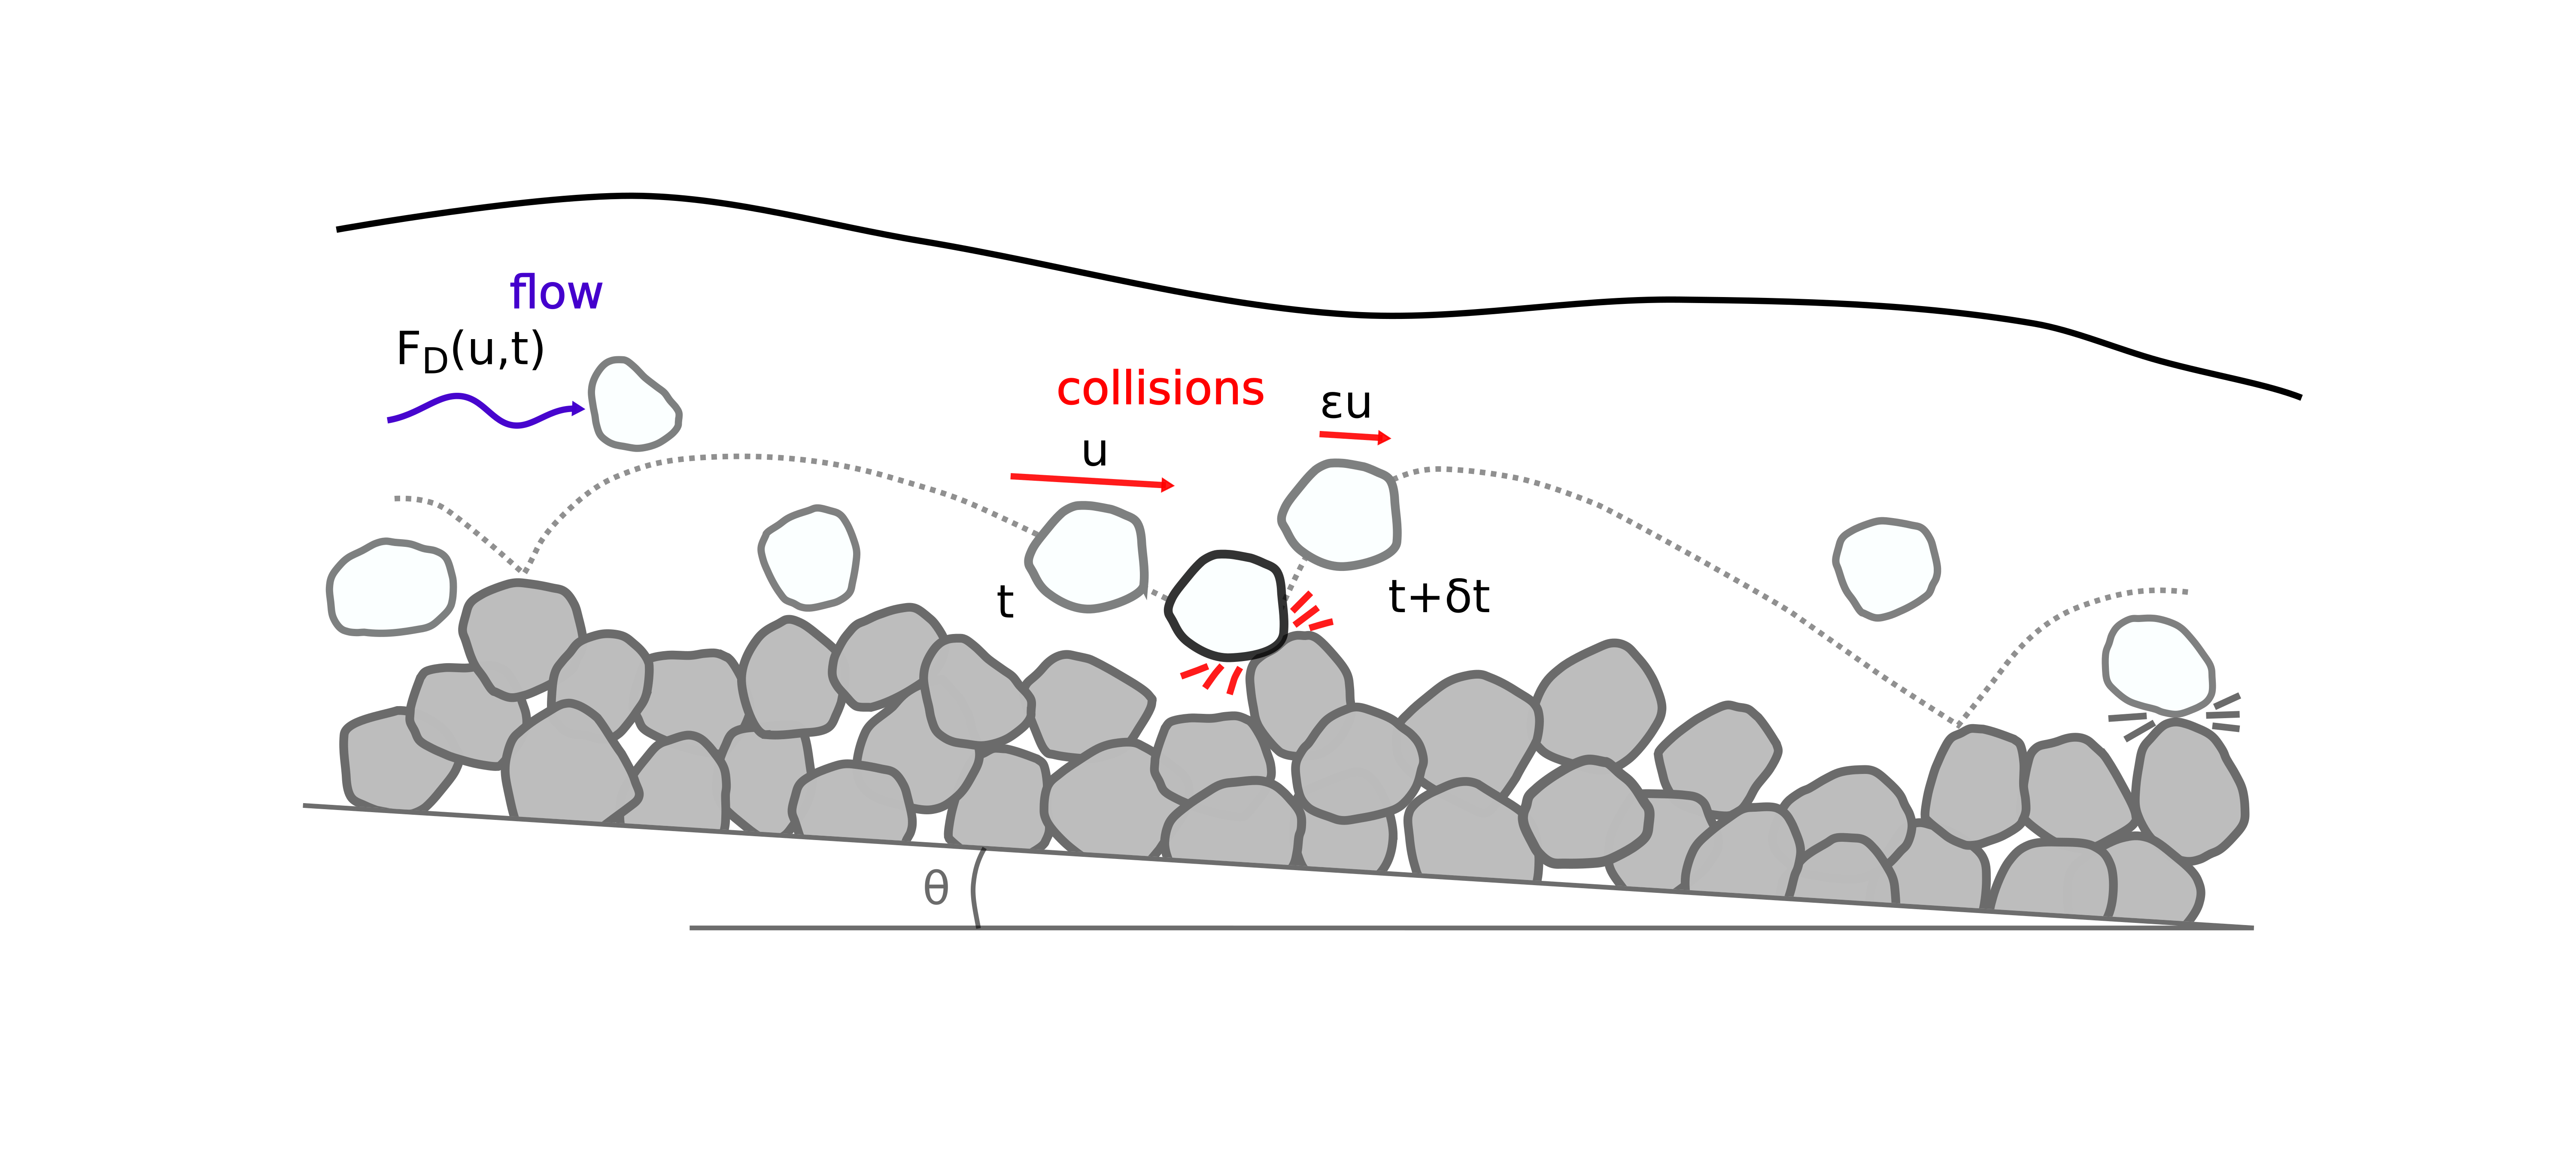
\includegraphics{./figures/ch5/Fig1Concept.png}}
	\caption{\DIFdelbeginFL \DIFdelFL{Definition sketch of rarefied }\DIFdelendFL \DIFaddbeginFL \DIFaddFL{Rarefied }\DIFaddendFL sediment transport \DIFdelbeginFL \DIFdelFL{with }\DIFdelendFL \DIFaddbeginFL \DIFaddFL{involves }\DIFaddendFL turbulent fluid drag and \DIFaddbeginFL \DIFaddFL{episodic }\DIFaddendFL particle-bed \DIFdelbeginFL \DIFdelFL{collision forces}\DIFdelendFL \DIFaddbeginFL \DIFaddFL{collisions}\DIFaddendFL . \DIFdelbeginFL \DIFdelFL{During saltation}\DIFdelendFL \DIFaddbeginFL \DIFaddFL{In the collision model of this chapter}\DIFaddendFL , pre-collisional streamwise velocities $u$ are transformed \DIFaddbeginFL \DIFaddFL{instantaneously }\DIFaddendFL to \DIFdelbeginFL \DIFdelFL{postcollisional }\DIFdelendFL \DIFaddbeginFL \DIFaddFL{post-collisional }\DIFaddendFL velocities $\ve u < u$.}
	\label{fig:fig1}
\end{figure}

Since the elasticity combines effects of particle shape and collision geometry and should vary from one collision to the next, the elasticity $\varepsilon$ is interpreted as a random variable, characterized by a statistical distribution $\rho(\varepsilon)$.
Some granular gas models have also included random elasticity \citep[e.g.][]{Serero2015}\DIFaddbegin \DIFadd{, but this topic has not been deeply explored in the literature}\DIFaddend .

Assuming that the number of collisions per unit time is $\nu$ and that the time intervals between subsequent particle-bed collisions are exponentially distributed \DIFdelbegin \DIFdel{\mbox{%DIFAUXCMD
\citep{Gordon1972}}\hspace{0pt}%DIFAUXCMD
}\DIFdelend \DIFaddbegin \DIFadd{\mbox{%DIFAUXCMD
\citep[e.g.][]{Gordon1972}}\hspace{0pt}%DIFAUXCMD
}\DIFaddend , the collision force in the downstream direction can be written as a Poisson pulse noise (\DIFdelbegin \DIFdel{sec}\DIFdelend \DIFaddbegin \DIFadd{Sec}\DIFaddend . \ref{sec:einflux}):
\be F_C(u,t) = - m u \sum_{k=1}^{N_\nu(t)}(1-\varepsilon_k)\delta(t-\tau_k). \label{eq:col} \ee
Here, $N_\nu(t)$ is the number of collisions in time $t$ (a Poisson random variable), the $\tau_k$ ($k=1,2,\dots$) are times at which collisions occur, and the $\varepsilon_k$ are the elasticity coefficients, drawn from the distribution $\rho(\varepsilon)$ characterizing the fraction of momentum lost in each particle-bed collision.
\DIFaddbegin \DIFadd{The time intervals $\Delta \tau_k = \tau_k-\tau_{k-1}$ between collisions are distributed as $P(\Delta \tau) = \nu \exp(-\nu\Delta \tau),$ so the number of collisions $n=N_\nu(t)$ in time $t$ is distributed as $P(n) = (\nu t)^n/n! \exp(-\nu t).$
}\DIFaddend This collision force is a sequence of random impulses which are proportional to the pre-collisional streamwise \DIFdelbegin \DIFdel{momentum}\DIFdelend \DIFaddbegin \DIFadd{momenta}\DIFaddend . This collision model should be adequate when the contact times between moving and resting particles are small compared to the times between collisions. These conditions \DIFdelbegin \DIFdel{are always }\DIFdelend \DIFaddbegin \DIFadd{should be }\DIFaddend satisfied for the \DIFdelbegin \DIFdel{idealized }\DIFdelend saltation trajectories depicted in \DIFdelbegin \DIFdel{figure }\DIFdelend \DIFaddbegin \DIFadd{Fig. }\DIFaddend \ref{fig:fig1}.

\subsection{Turbulent fluid forces}
\DIFaddbegin 

\DIFaddend Fluid forces on \DIFdelbegin \DIFdel{a coarse particle in a viscous flow depend on the Reynolds number $\Re_p = d V/\nu$ defined by }\DIFdelend \DIFaddbegin \DIFadd{coarse particles are parameterized by the particle Reynolds number $\Rey_p = V d/\lambda$, involving }\DIFaddend the particle size $d$, slip velocity $V$ between particle and fluid, and kinematic viscosity \DIFdelbegin \DIFdel{$\nu$}\DIFdelend \DIFaddbegin \DIFadd{$\lambda$}\DIFaddend .
These forces have been calculated \DIFdelbegin \DIFdel{analytically }\DIFdelend from the Navier-Stokes equations for \DIFdelbegin \DIFdel{vanishing $\Re_p$ and include acceleration, history, and velocity-dependent drag }\DIFdelend \DIFaddbegin \DIFadd{spherical particles at small (or vanishing) $\Rey_p$ and include drag, virtual mass, buoyancy, fluid pressure gradient, Basset history integral, Saffman lift, and Magnus lift }\DIFaddend terms \citep{Hjelmfelt1966, Maxey1983, Auton1987}.
At realistic \DIFdelbegin \DIFdel{$\Re_p$}\DIFdelend \DIFaddbegin \DIFadd{$\Rey_p$}\DIFaddend , analytical results \DIFdelbegin \DIFdel{are }\DIFdelend \DIFaddbegin \DIFadd{for the fluid forces on a particle remain }\DIFaddend inaccessible, so it is standard \DIFdelbegin \DIFdel{to include }\DIFdelend \DIFaddbegin \DIFadd{practice to introduce }\DIFaddend empirical corrections to the small \DIFdelbegin \DIFdel{$\Re_p$ formulas \mbox{%DIFAUXCMD
\citep{Schmeeckle2007,Clift1978}}\hspace{0pt}%DIFAUXCMD
.
A dominant contribution to the downstream drag force $F_D$ on nearly spherical particles at large $\Re_p$ can be written 
$F_D = \frac{\pi}{8}
\rho_f d^2 C_D(\Re_p) |V|V$, }\DIFdelend \DIFaddbegin \DIFadd{$\Rey_p$ formulas \mbox{%DIFAUXCMD
\citep[e.g.][]{Clift1978,Schmeeckle2007}}\hspace{0pt}%DIFAUXCMD
.
}

\DIFadd{Our understanding of the fluid forces remains incomplete.
Existing formulas were derived in the absence of boundaries, so it is unclear how these formulas should be modified near the bed.
Even ignoring this complication, the added mass and Basset forces are difficult to compute and therefore impractical to include in analytical models.
These challenges require us to adopt the most complex expressions of the fluid forces that are compatible with our modeling goals \mbox{%DIFAUXCMD
\citep[e.g.][]{Michaelides1997,Armenio2001}}\hspace{0pt}%DIFAUXCMD
.
From this same requirement, a majority of bedload transport models include fluid drag (and possibly pressure gradient) terms as the only force driving the downstream movement of bedload particles \mbox{%DIFAUXCMD
\citep{Ancey2014,Fan2014,Schmeeckle2014,Gonzalez2017,Elghannay2017}}\hspace{0pt}%DIFAUXCMD
.
}

\DIFadd{The downstream drag force with the $\Rey_p$ correction is usually written 
}\be \DIFadd{F_D = \frac{\pi}{8} \rho_f d^2 C_D(}\Rey\DIFadd{_p) |V|V, }\label{eq:draggy}\ee
\DIFaddend where $\rho_f$ is the fluid density, $d$ is the particle diameter, \DIFdelbegin \DIFdel{$C_D(\Re_p)$ }\DIFdelend \DIFaddbegin \DIFadd{$C_D(\Rey_p)$ }\DIFaddend is an empirical drag coefficient, and $V = U-u$ is the slip velocity \DIFdelbegin \DIFdel{between the }\DIFdelend \DIFaddbegin \DIFadd{calculated as the difference of }\DIFaddend fluid ($U$) and particle ($u$) velocities \citep{Coleman1967, Schmeeckle2007, Dwivedi2012}.
\DIFdelbegin \DIFdel{In this study, I leave out acceleration and history terms for analytical tractability, although they are certainly relevant in coarse sediment transport \mbox{%DIFAUXCMD
\citep{Michaelides1997,Armenio2001}}\hspace{0pt}%DIFAUXCMD
.
}\DIFdelend \DIFaddbegin \DIFadd{Experiments on stationary particles indicate that drag forces fluctuate rapidly and lie on wide Gaussian-like distributions \mbox{%DIFAUXCMD
\citep{Hofland2006,Schmeeckle2007,Dwivedi2010,Celik2014}}\hspace{0pt}%DIFAUXCMD
.
The drag forces on moving particles have not been experimentally measured, but even in globally steady flow conditions, slip velocities are expected to fluctuate due to particle acceleration, fluid turbulence, passage of other moving particles, and vertical movement of particles within the flow profile.
The nonlinearity in Eq. \ref{eq:draggy} will amplify slip velocity fluctuations, generating large and erratic drag force variations that only add to the undetermined contributions of the neglected fluid forces.
}\DIFaddend 

\DIFdelbegin \DIFdel{Drag forces have been argued to fluctuate rapidly compared to the inertial response times of submerged grains \mbox{%DIFAUXCMD
\citep{Fan2014}}\hspace{0pt}%DIFAUXCMD
, and the magnitude of drag fluctuationshas been observed to follow a Gaussian distribution \mbox{%DIFAUXCMD
\citep{Hofland2006,Schmeeckle2007,Dwivedi2010,Celik2014}}\hspace{0pt}%DIFAUXCMD
.
These ideas allow two major simplifications of the above drag force.
First, the drag can be split into quasi-steady and fluctuating components \mbox{%DIFAUXCMD
\citep{Michaelides1997}}\hspace{0pt}%DIFAUXCMD
, and second, drag fluctuations can be modelled }\DIFdelend \DIFaddbegin \DIFadd{Here I assume with earlier computational \mbox{%DIFAUXCMD
\citep{Schmeeckle2014,Gonzalez2017,Elghannay2017} }\hspace{0pt}%DIFAUXCMD
and analytical \mbox{%DIFAUXCMD
\citep[e.g.][]{Ancey2014,Fan2014} }\hspace{0pt}%DIFAUXCMD
models of bedload transport that fluid drag is the primary force driving sediment particles downstream. I further assume with \mbox{%DIFAUXCMD
\citet{Fan2014} }\hspace{0pt}%DIFAUXCMD
and \mbox{%DIFAUXCMD
\citet{Ancey2014} }\hspace{0pt}%DIFAUXCMD
that the fluctuating component of this force can be represented by }\DIFaddend a Gaussian white noise\DIFdelbegin \DIFdel{, where the fluctuations are symmetric, the autocorrelation time is negligible, and the strength of fluctuations is described by a diffusivity $D$ \mbox{%DIFAUXCMD
\citep{Fan2014,Ancey2014}}\hspace{0pt}%DIFAUXCMD
.
Defining $\bar{V}$ as a representative slip velocity to be specified more carefully later,  }\DIFdelend \DIFaddbegin \DIFadd{.
This latter assumption is justified insofar as drag forces fluctuate rapidly compared to the inertial response times of particles and the timescales over which particles change height within the flow profile.
Defining }\DIFaddend $\bar{C}_D$ as the empirical drag coefficient evaluated at \DIFdelbegin \DIFdel{this slip velocity, }\DIFdelend \DIFaddbegin \DIFadd{$\bar{V}$ }\DIFaddend and $\xi(t)$ as a Gaussian white noise of mean $0$ and variance $1$ \DIFdelbegin \DIFdel{\mbox{%DIFAUXCMD
\citep{Gardiner1983}}\hspace{0pt}%DIFAUXCMD
}\DIFdelend \DIFaddbegin \DIFadd{\mbox{%DIFAUXCMD
\citep[e.g.][]{Gardiner1983}}\hspace{0pt}%DIFAUXCMD
}\DIFaddend , the fluid drag \DIFdelbegin \DIFdel{can be written
}\DIFdelend \DIFaddbegin \DIFadd{force considered in this chapter is
}\DIFaddend \be F_D(t) = \Gamma + \sqrt{2 D } \eta(t), \label{eq:drag}\ee
where $\Gamma = \frac{\pi}{8}
\rho_f d^2 \bar{C}_D \bar{V}^2$ is the steady component of the drag.
\DIFaddbegin \DIFadd{Although this representation of the fluid forces is a simplified approximation, it is similar to the representations used in earlier stochastic models in that it has no dependence on the vertical structure of the flow \mbox{%DIFAUXCMD
\citep[e.g.][]{Fan2014,Ancey2014}}\hspace{0pt}%DIFAUXCMD
. This level of simplification is required for an analytically tractable model of bedload particle velocities \mbox{%DIFAUXCMD
\citep[e.g.][]{Michaelides1997}}\hspace{0pt}%DIFAUXCMD
.
}\DIFaddend 

\subsection{Langevin equation for collisional bedload transport}

With the above forces, the Langevin equation $m\dot{u}(t) = F_D(t) + F_C(t)$ for the sediment dynamics \DIFaddbegin \DIFadd{in the downstream direction }\DIFaddend becomes
\be m \dot{u}(t) = \Gamma + \sqrt{2D}\eta(t) - m u(t) \xi_{\nu, \ve}(t). \label{eq:langevin} \ee
This equation replaces the steady friction terms of earlier models with an episodic term, designed to provide a more realistic representation of particle-bed collisions.
Mathematically, \DIFdelbegin \DIFdel{equation }\DIFdelend \DIFaddbegin \DIFadd{Eq. }\DIFaddend \ref{eq:langevin} is a Langevin-like equation representing a jump-diffusion process \citep{Daly2006} with multiplicative Poisson noise \citep{Dubkov2016,Denisov2009}. 
Collisions introduce \DIFdelbegin \DIFdel{``jumps" in velocity while turbulent generates "diffusion"}\DIFdelend \DIFaddbegin \DIFadd{velocity jumps while turbulence generates velocity diffusion}\DIFaddend . The collision term is \DIFdelbegin \DIFdel{"multiplicative " }\DIFdelend \DIFaddbegin \DIFadd{multiplicative }\DIFaddend in the sense that $u$ multiplies the Poisson noise \DIFaddbegin \DIFadd{$\xi_{\nu,\ve}(t)$}\DIFaddend .

\DIFdelbegin \DIFdel{Equations like }\DIFdelend \DIFaddbegin \DIFadd{Models like Eq. }\DIFaddend \ref{eq:langevin} have long been studied in the stochastic physics literature \citep{Hanggi1978,VanDenBroeck1983}, but solving such equations remains extremely challenging \citep{Daly2010,Mau2014,Dubkov2019}.
One issue is that multiplicative white noises imply the prescription dilemma of stochastic calculus \citep{Risken1989,Gardiner1983}, meaning \DIFaddbegin \DIFadd{Eq. }\DIFaddend \ref{eq:langevin} is not defined without further specifying an integration rule \citep{Suweis2011}.
Here, the \DIFdelbegin \DIFdel{Ito }\DIFdelend \DIFaddbegin \DIFadd{It\^{o} }\DIFaddend interpretation (lower endpoint integration rule) is the physical choice the energy dissipated by collisions depends strictly on pre-collisional velocities, not post-collisional \citep[e.g.][]{Gardiner1983}\DIFdelbegin \DIFdel{since}\DIFdelend .
Given this integration rule, the remaining issues are to obtain the master equation characterizing the ensemble of velocities defined by \DIFaddbegin \DIFadd{Eq. }\DIFaddend \ref{eq:langevin}, and then to solve this equation for the velocity distribution \DIFdelbegin \DIFdel{$P(u)$}\DIFdelend \DIFaddbegin \DIFadd{$P(u,t)$}\DIFaddend .

\subsection{\DIFdelbegin \DIFdel{Chapman-Komogorov }\DIFdelend \DIFaddbegin \DIFadd{Chapman-Kolmogorov }\DIFaddend equation and particle-bed collision integral}

The equation governing the streamwise velocity distribution $P(u,t)$ is derived in \DIFdelbegin \DIFdel{appendix section }\DIFdelend \DIFaddbegin \DIFadd{the appendix Sec. }\DIFaddend \ref{sec:langmasterderiv} with a limiting procedure, providing
\be \nu^{-1}\partial_t P(u,t) = - \tilde{\Gamma} \partial_u P(u,t) + \tilde{D} \partial_u^2 P(u,t) + I_c(u,t). \label{eq:master} \ee
\DIFdelbegin \DIFdel{In this equation, I introduced the scaled }\DIFdelend \DIFaddbegin \DIFadd{The }\DIFaddend parameters $\tilde{\Gamma} = \Gamma/(\nu m)$ and $\tilde{D} = D/(\nu m)$ \DIFdelbegin \DIFdel{that }\DIFdelend scale the steady and fluctuating components of the fluid force against the collision rate $\nu$. The term
\be \DIFdelbegin \DIFdel{\mathcal{I}}\DIFdelend \DIFaddbegin \DIFadd{I}\DIFaddend _c(u,t) = - P(u,t) + \int_0^1 \frac{d\ve}{\ve}P\big(\frac{u}{\ve},t \big) \rho(\ve) \label{eq:colint} \ee
is a ``collision integral" term representing particle-bed collisions.

\DIFdelbegin \DIFdel{Equation }\DIFdelend \DIFaddbegin \DIFadd{Eq. }\DIFaddend \ref{eq:master} is a nonlocal extension of the Fokker-Planck equation used in earlier \DIFdelbegin \DIFdel{bed load }\DIFdelend \DIFaddbegin \DIFadd{bedload }\DIFaddend models \citep{Fan2014,Ancey2014}. 
Nonlocality is introduced by the collision integral \DIFaddbegin \DIFadd{of Eq. }\DIFaddend \ref{eq:colint} which transfers probability from higher pre-collisional velocities $u/\varepsilon$ to lower post-collisional velocities $u$.
This term is analogous to the collision integral within the Boltzmann equation of kinetic theory \citep{Duderstadt1979, Brilliantov2004}. Physically, it corresponds to binary collisions between particles having different masses and random \DIFdelbegin \DIFdel{resitution coefficients \mbox{%DIFAUXCMD
\cite{Serero2015} }\hspace{0pt}%DIFAUXCMD
}\DIFdelend \DIFaddbegin \DIFadd{restitution coefficients \mbox{%DIFAUXCMD
\citep[cf.][]{Serero2015} }\hspace{0pt}%DIFAUXCMD
}\DIFaddend in the limit that the mass of one particle (here, the particle resting on the bed) diverges to infinity.
Mathematically, the collision integral represents the probability distribution of the product between the elasticity $\varepsilon$ and the downstream momentum \DIFdelbegin \DIFdel{$m u$ \mbox{%DIFAUXCMD
\citep[c.f.][]{Feller1968}}\hspace{0pt}%DIFAUXCMD
}\DIFdelend \DIFaddbegin \DIFadd{$(p = m u)$, considering them as uncorrelated random variables \mbox{%DIFAUXCMD
\citep[cf.][]{Feller1968}}\hspace{0pt}%DIFAUXCMD
}\DIFaddend .


Owing to its nonlocality, \DIFdelbegin \DIFdel{equation }\DIFdelend \DIFaddbegin \DIFadd{Eq. }\DIFaddend \ref{eq:master} does not admit analytical solutions as is, so further approximation is necessary.
\DIFdelbegin \DIFdel{Assuming }\DIFdelend \DIFaddbegin \DIFadd{To make progress, I assume }\DIFaddend the distribution of elasticity $\rho(\varepsilon)$ is sharply peaked at some most common (mode) value $\varepsilon'$ \DIFdelbegin \DIFdel{, which is the case in experiments of rigid body collisions \mbox{%DIFAUXCMD
\citep{Glielmo2014}}\hspace{0pt}%DIFAUXCMD
, allows }\DIFdelend \DIFaddbegin \DIFadd{to allow }\DIFaddend for a Kramers-Moyal type expansion of the particle-bed collision integral \DIFdelbegin \DIFdel{\mbox{%DIFAUXCMD
\citep{Gardiner1983}}\hspace{0pt}%DIFAUXCMD
.
}\DIFdelend \DIFaddbegin \DIFadd{\mbox{%DIFAUXCMD
\citep[e.g.][]{Gardiner1983}}\hspace{0pt}%DIFAUXCMD
.
Such a mode value in the collision elasticity distribution is present in experiments on rigid body collisions \mbox{%DIFAUXCMD
\citep{Glielmo2014}}\hspace{0pt}%DIFAUXCMD
.
For particle-bed collisions of bedload, a modal elasticity is also expected since experiments indicate a most common collision geometry \mbox{%DIFAUXCMD
\citep[e.g.][]{Gordon1972,Martin2013}}\hspace{0pt}%DIFAUXCMD
.
}

\DIFaddend Expanding all terms in the integrand except $\rho(\varepsilon)$ provides
\be \DIFdelbegin \DIFdel{\mathcal{I}}\DIFdelend \DIFaddbegin \DIFadd{I}\DIFaddend _c(u,t) = -P(u,t) + \frac{1}{\varepsilon'}P\big(\frac{u}{\ve'},t \big) + \sum_{k=1}^\infty \frac{\alpha_k }{k!}(\ve - \ve')^k \Big[\frac{1}{\ve}P\big(\frac{u}{\ve}\big)\Big]^{(k)}\Big|_{\ve=\ve'},\label{eq:expansion}\ee
where the $\alpha_k = \int_0^1 d\ve \rho(\ve) (\ve-\ve')^k $ are the central moments of $\ve$ around the \DIFdelbegin \DIFdel{mode }\DIFdelend \DIFaddbegin \DIFadd{modal }\DIFaddend elasticity $\ve'$ and the superscript $(k)$ denotes the $k$th derivative.

In what follows, I drop all but the first two terms in this expansion to obtain the leading order contribution of particle-bed collisions to the velocity distribution.
Higher orders could always be included later by perturbation theory \DIFdelbegin \DIFdel{\mbox{%DIFAUXCMD
\citep{Morse1953}}\hspace{0pt}%DIFAUXCMD
}\DIFdelend \DIFaddbegin \DIFadd{\mbox{%DIFAUXCMD
\citep{Morse1953a}}\hspace{0pt}%DIFAUXCMD
}\DIFaddend .
I solve the resulting approximate equation in steady-state, when $\partial P(u,t)/\partial t = 0$. \DIFdelbegin \DIFdel{Equation }\DIFdelend \DIFaddbegin \DIFadd{Eq. }\DIFaddend \ref{eq:master} indicates that this solution will be a good approximation to the time-dependent problem when particle motions generally survive multiple collisions ($t\gg \nu^{-1}$).

\section{Results}
\label{sec:langresults}

\subsection{Derivation of the bedload velocity distribution}
\label{sec:langsolution}
Hereafter I drop the prime on the most common streamwise restitution coefficient $\ve'$.
With the truncation to two terms, \DIFdelbegin \DIFdel{equation }\DIFdelend \DIFaddbegin \DIFadd{Eq. }\DIFaddend \ref{eq:master} gives 
\be 0 = -\tilde{\Gamma}\partial_u P(u) + \tilde{D}\partial_u^2 P(u) -P(u) + \frac{1}{\ve} P\big(\frac{u}{\ve}\big),\label{eq:governer} \ee
which is an advanced functional differential equation. This equation is ``functional" in the sense that it is nonlocal in velocity due to the last term on the right hand side, and it is ``advanced" in that $u/\ve$ is advanced beyond the argument $u$ involved in the rest of this equation (since $0<\ve<1$).
Such equations \DIFaddbegin \DIFadd{have }\DIFaddend seen some attention in the mathematics literature, where they are sometimes called pantograph equations \citep{Hall1989, Kim1998,Zaidi2015}.

In the appendix \DIFdelbegin \DIFdel{section \ref{sec:langsteadyderiv} I solve equation \ref{eq:governer} using }\DIFdelend \DIFaddbegin \DIFadd{Sec. \ref{sec:langsteadyderiv} Eq. \ref{eq:governer} is solved with }\DIFaddend Laplace transforms, providing
\begin{multline} P(u) = \frac{\theta(-u)}{K_+}\sum_{l=0}^\infty \frac{\ve^{-l}e^{\lambda_+\ve^{-l}u}}{\prod_{m=1}^l(-\tilde{D} \lambda_+^2 \ve^{-2m} + \tilde{\Gamma} \lambda_+ \ve^{-m} + 1) } 
	\\+ \frac{\theta(u)}{K_-}\sum_{l=0}^\infty \frac{\ve^{-l}e^{\lambda_-\ve^{-l}u}}{\prod_{m=1}^l(- \tilde{D} \lambda_-^2 \ve^{-2m} + \tilde{\Gamma} \lambda_- \ve^{-m} + 1) } \label{eq:steadystate}. \end{multline}
The factors $\lambda_\pm$ are defined in appendix \DIFdelbegin \DIFdel{equations }\DIFdelend \DIFaddbegin \DIFadd{Eq. }\DIFaddend \ref{eq:lambdas}. They are proportional to $\tilde{\Gamma}/\tilde{D}$. 
The normalization factors \DIFdelbegin \DIFdel{are }\DIFdelend $K_\pm$ are 
\be K_\pm = \tilde{D}(\lambda_+-\lambda_-)\prod_{l=1}^\infty (- \tilde{D}\lambda_\pm^2 \ve^{2l} +\tilde{\Gamma} \lambda_\pm \ve^{l} + 1). \ee
Although this velocity distribution has a complex mathematical structure, one can verify that this is a normalized probability distribution ($\int du P(u) = 1$) which has very simple limiting behaviors as the mode elasticity $\ve$ approaches fully elastic ($\ve=1$) and inelastic ($\ve = 0$) values.
\DIFdelbegin \DIFdel{The complexity of this result is not surprising given how few analytical solutions are available in granular gas theories with similar nonlocal collision integrals \mbox{%DIFAUXCMD
\citep[e.g.][]{Brilliantov2004}}\hspace{0pt}%DIFAUXCMD
.
}\DIFdelend 

It is possible to derive the moments of this probability distribution by multiplying \DIFaddbegin \DIFadd{Eq. }\DIFaddend \ref{eq:governer} by $u$, integrating, and then solving the resulting moment evolution equations \DIFdelbegin \DIFdel{\mbox{%DIFAUXCMD
\citep[c.f.][]{Cox1965}}\hspace{0pt}%DIFAUXCMD
}\DIFdelend \DIFaddbegin \DIFadd{\mbox{%DIFAUXCMD
\citep[e.g.][]{Cox1965}}\hspace{0pt}%DIFAUXCMD
}\DIFaddend .
These calculations are provided in \DIFdelbegin \DIFdel{appendix section }\DIFdelend \DIFaddbegin \DIFadd{the appendix Sec. }\DIFaddend \ref{sec:langmoments}, where the mean bedload velocity is derived as
\be \langle u \rangle = \frac{\Gamma}{\nu(1-\ve)} = \DIFdelbegin \DIFdel{\frac{\gamma}{1-\ve}}\DIFdelend \DIFaddbegin \DIFadd{\frac{\tilde{\Gamma}}{1-\ve}}\DIFaddend . \label{eq:meanu}\ee
This result scales linearly with the mean fluid drag and nonlinearly with the rate and typical elasticity of collisions, indicating a strong influence of particle collisions on bedload velocities.
The second moment is
\be \langle u^2 \rangle = 2 \DIFdelbegin \DIFdel{\frac{d + \gamma \langle u \rangle}{1-\ve^2}}\DIFdelend \DIFaddbegin \DIFadd{\frac{\tilde{D} + \tilde{\Gamma} \langle u \rangle}{1-\ve^2}}\DIFaddend , \ee
leading to the velocity variance ($\sigma_u^2 = \bra u^2 \ket - \bra u \ket ^2 $)
\be \sigma_u^2 = \DIFdelbegin \DIFdel{\frac{2 d + \gamma^2}{1-\ve^2}}\DIFdelend \DIFaddbegin \DIFadd{\frac{2 \tilde{D}+ \tilde{\Gamma}^2}{1-\ve^2}}\DIFaddend . \label{eq:varu}\ee
This result demonstrates that \DIFaddbegin \DIFadd{within the model, }\DIFaddend velocity fluctuations originate from both the steady and fluctuating components of the flow forces, yet the variance is linear in these factors and is therefore relatively insensitive to the fluid flow.
This is consistent with the \DIFdelbegin \DIFdel{remarkable similarities sometimes visible }\DIFdelend \DIFaddbegin \DIFadd{similarities apparent }\DIFaddend between viscous and turbulent flow experiments \citep[e.g.][]{Charru2004,Lajeunesse2010}.
In contrast, particle velocity fluctuations in \DIFdelbegin \DIFdel{equation }\DIFdelend \DIFaddbegin \DIFadd{Eq. }\DIFaddend \ref{eq:varu} depend sharply on the parameters representing particle-bed collisions, suggesting collisions \DIFdelbegin \DIFdel{are }\DIFdelend \DIFaddbegin \DIFadd{could be }\DIFaddend the leading control on particle velocity fluctuations.

\DIFdelbegin \DIFdel{Figure }\DIFdelend \DIFaddbegin \DIFadd{Fig. }\DIFaddend \ref{fig:fig2} depicts the velocity characteristics of particles for different realizations of the fluid and collisional forces.
\begin{figure}
	\centerline{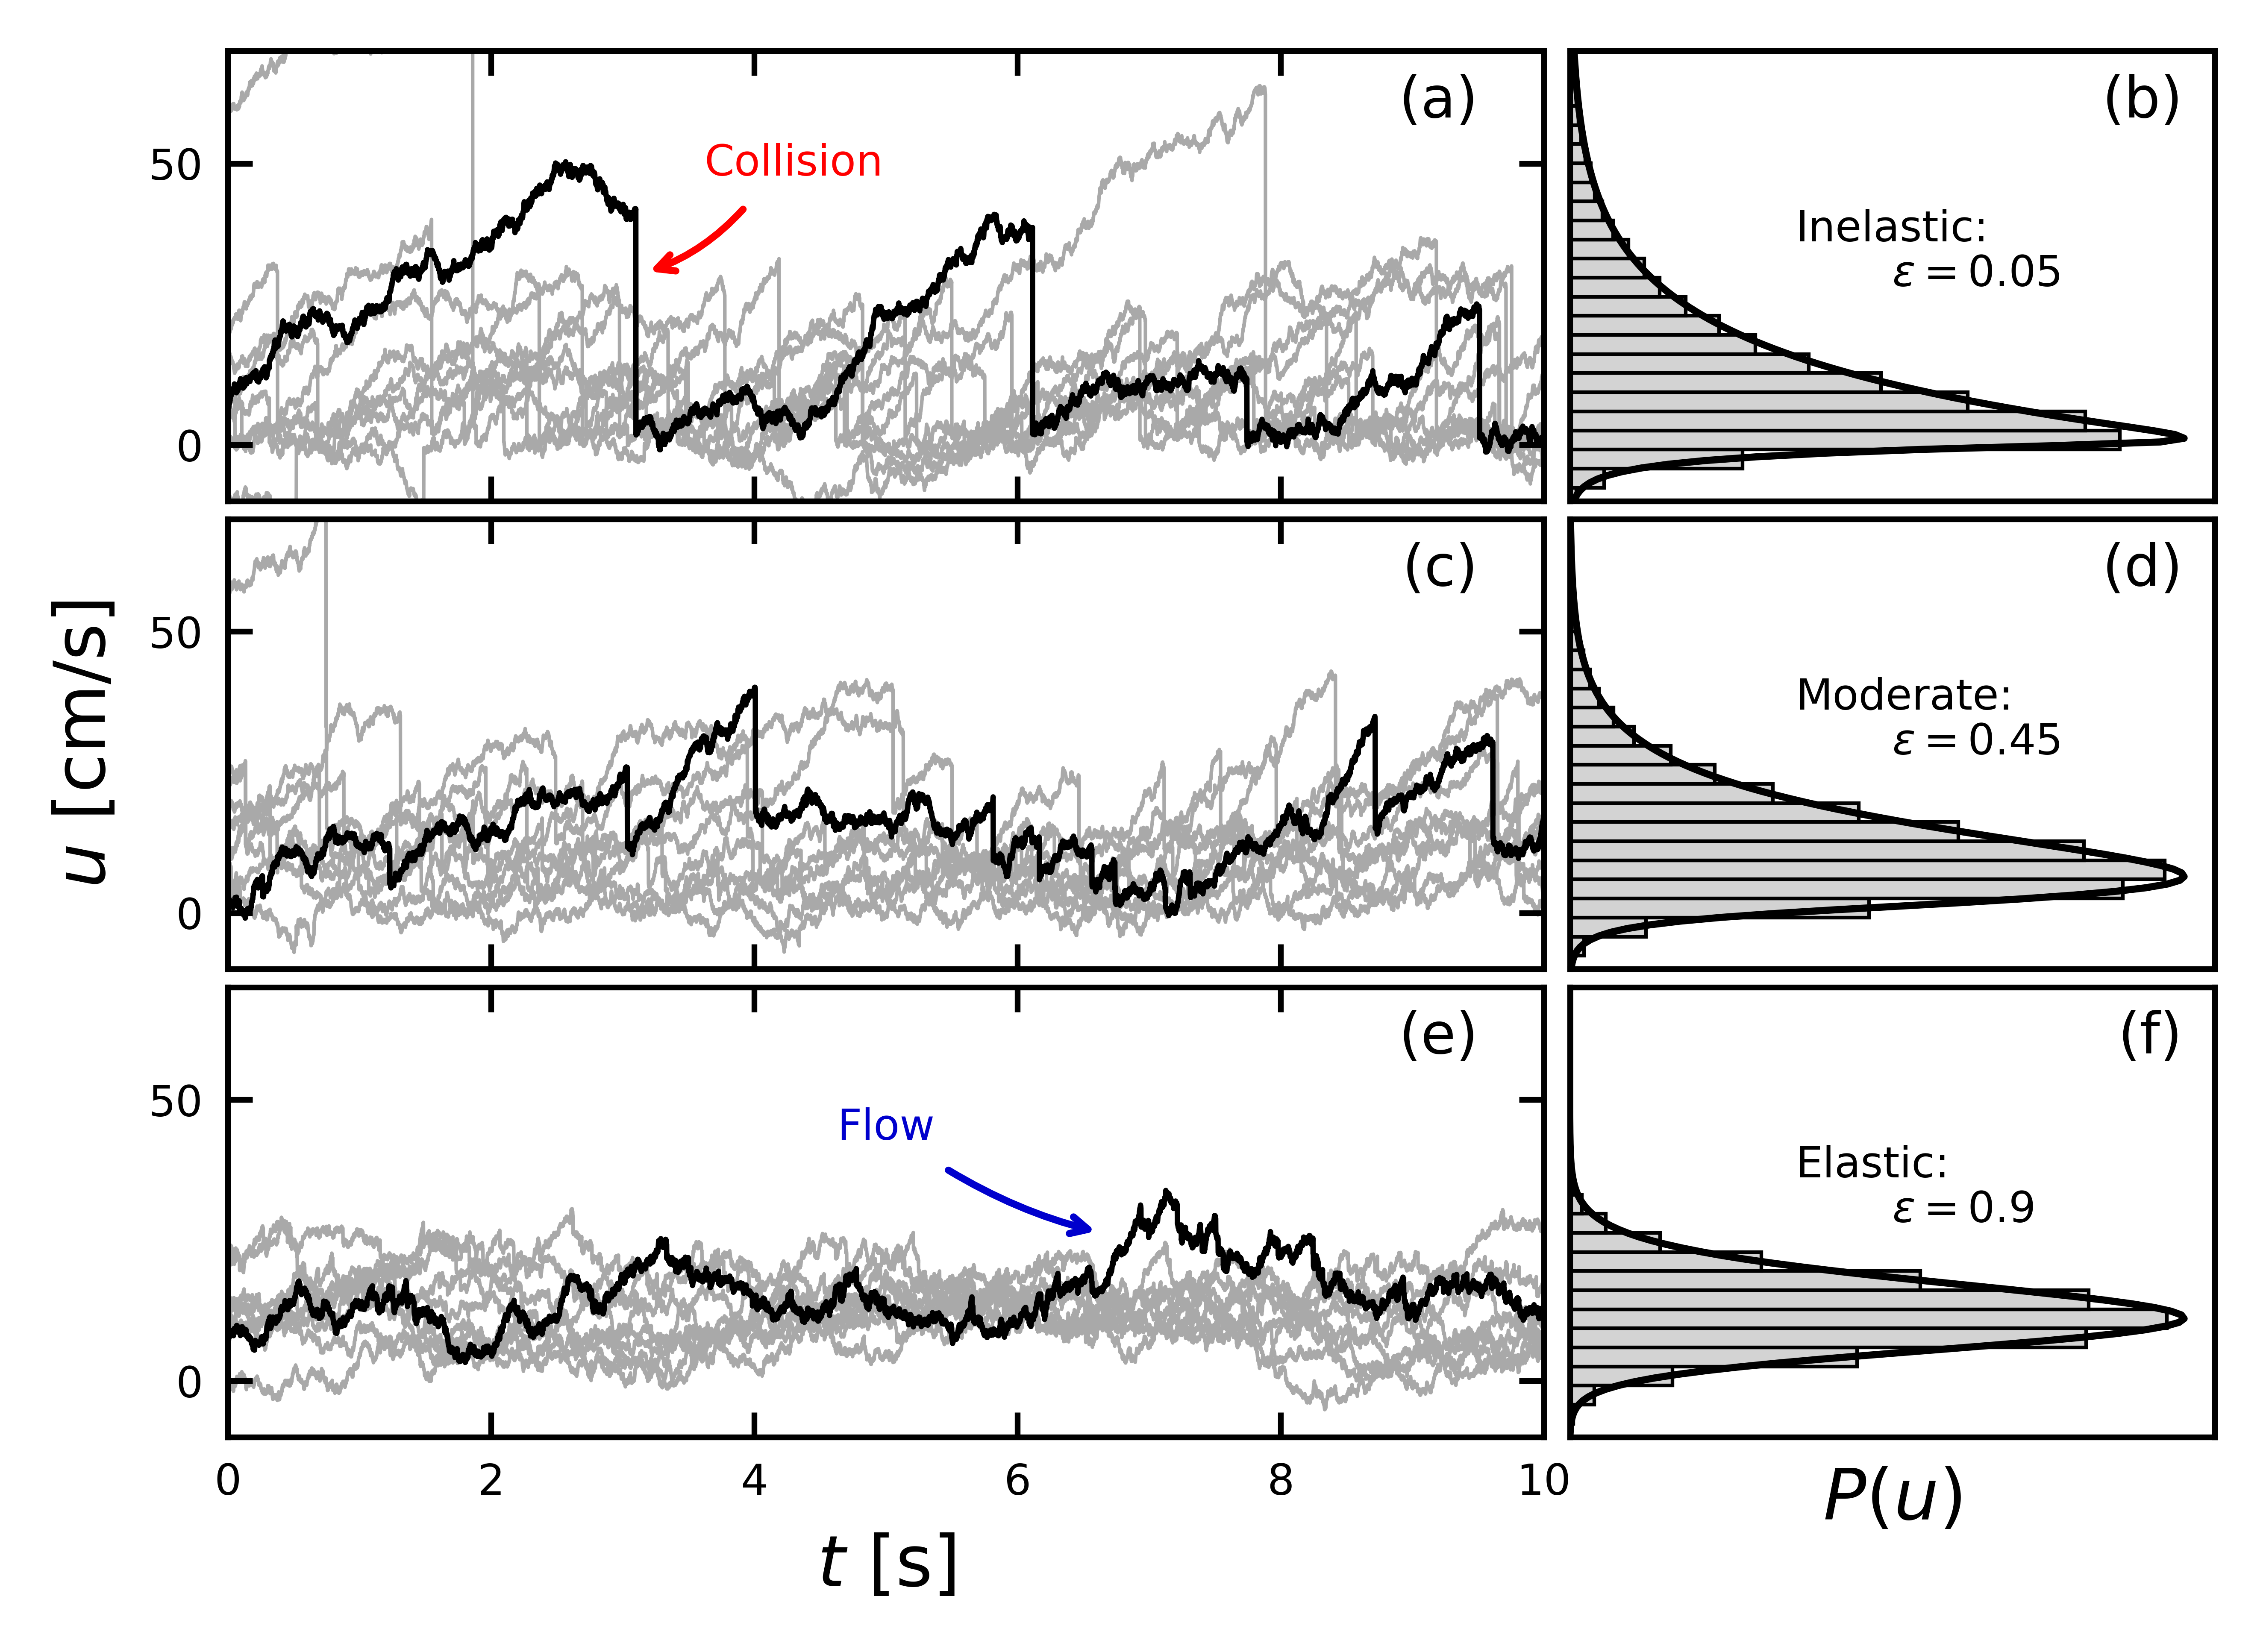
\includegraphics{./figures/ch5/Fig2pdfs.png}}
	\caption{Left and right panels are paired. Left panels show velocity realizations as gray traces. Velocities are calculated from Monte Carlo simulations. Individual realizations are singled out as black traces. Particle-bed collisions imply sudden downward-velocity jumps. Flow forces generate fluctuating positive accelerations between collisions. Right panels show simulated histograms of particle velocities and exact solutions from \DIFdelbeginFL \DIFdelFL{equation }\DIFdelendFL \DIFaddbeginFL \DIFaddFL{Eq. }\DIFaddendFL \ref{eq:steadystate}. As \DIFaddbeginFL \DIFaddFL{the }\DIFaddendFL elasticity $\ve$ varies, the particle velocity distributions interpolate between exponential (inelastic) and Gaussian (elastic) forms.}
	\label{fig:fig2}
\end{figure}
\DIFdelbegin \DIFdel{This figure }\DIFdelend \DIFaddbegin \DIFadd{Fig. \ref{fig:fig2} }\DIFaddend reveals an apparent transition from exponential-like to Gaussian-like velocity distributions as collisions vary from more inelastic ($\ve \rightarrow 0$) to more elastic ($\ve \rightarrow 1$). In between, the full distribution \DIFaddbegin \DIFadd{Eq. }\DIFaddend \ref{eq:steadystate} resembles a Gamma distribution, although it is represented by \DIFdelbegin \DIFdel{equation }\DIFdelend \DIFaddbegin \DIFadd{Eq. }\DIFaddend \ref{eq:steadystate}, not a Gamma distribution.


\subsection{Exponential and Gaussian regimes: \DIFdelbegin \DIFdel{limits }\DIFdelend \DIFaddbegin \DIFadd{Limits }\DIFaddend to earlier work}
\label{sec:langmodelcomparison}

In fact, the apparent transition from exponential to Gaussian in \DIFdelbegin \DIFdel{figure }\DIFdelend \DIFaddbegin \DIFadd{Fig. }\DIFaddend \ref{fig:fig2} can be demonstrated \DIFdelbegin \DIFdel{from equation }\DIFdelend \DIFaddbegin \DIFadd{analytically from Eq. }\DIFaddend \ref{eq:steadystate}. Despite its complex appearance, simple Gaussian and exponential forms derive from this equation as exact mathematical limits.
When particle-bed collisions are completely inelastic (\DIFdelbegin \DIFdel{$\ne = 0$), }\DIFdelend \DIFaddbegin \DIFadd{$\ve = 0$), Eq. }\DIFaddend \ref{eq:steadystate} becomes an exponential distribution, and when they are completely elastic (\DIFdelbegin \DIFdel{$\nu = 1$), }\DIFdelend \DIFaddbegin \DIFadd{$\ve = 1$), Eq. }\DIFaddend \ref{eq:steadystate} becomes Gaussian.
\DIFdelbegin \DIFdel{Figure }\DIFdelend \DIFaddbegin \DIFadd{Fig. }\DIFaddend \ref{fig:fig3} demonstrates in detail the approach of the distribution toward these limits.
\begin{figure}
	\centerline{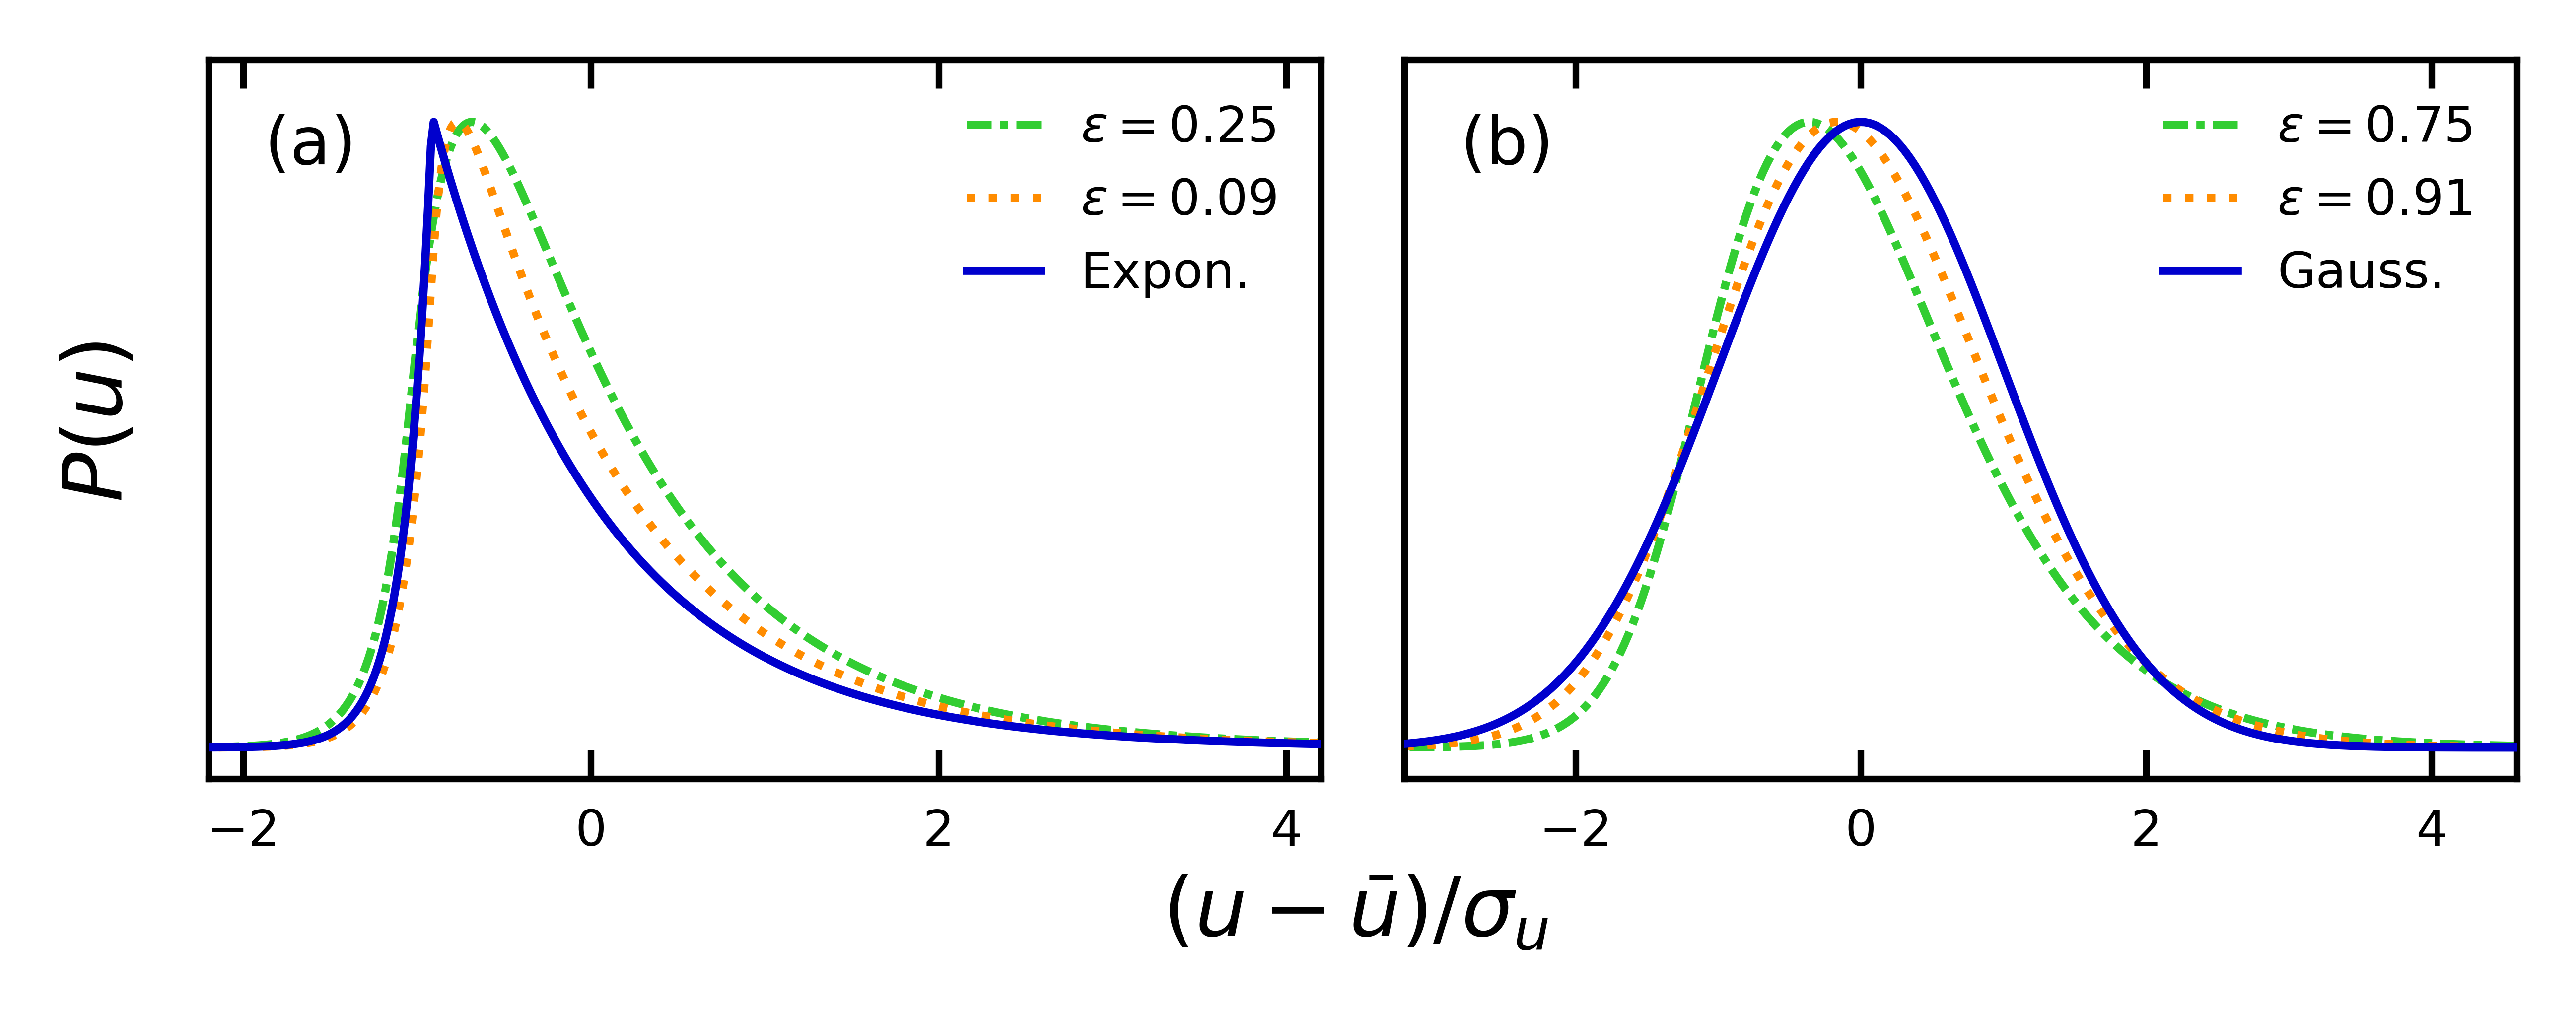
\includegraphics{./figures/ch5/Fig3asymptotic.png}}
	\caption{The particle velocity distribution approaches an exponential distribution in \DIFaddbeginFL \DIFaddFL{panel }\DIFaddendFL (a) as particle-bed collisions become extremely elastic ($\ve \rightarrow 1$), and it approaches a Gaussian in \DIFaddbeginFL \DIFaddFL{panel }\DIFaddendFL (b) as they become extremely inelastic ($\ve \rightarrow 0$). On the abscissa, the mean sediment velocity is standardized by its mean $\bar{u}$ and standard deviation $\sigma_u$. }
	\label{fig:fig3}
\end{figure}

The exponential limit of \DIFaddbegin \DIFadd{Eq. }\DIFaddend \ref{eq:steadystate} as $\ve \rightarrow 0$ is easy to see. Taking $\ve \rightarrow 0 $ in \DIFaddbegin \DIFadd{Eq. }\DIFaddend \ref{eq:steadystate}, all terms in the series except for \DIFdelbegin \DIFdel{that with }\DIFdelend \DIFaddbegin \DIFadd{the one at }\DIFaddend $l=0$ become exponentially small, leaving behind the same two-sided exponential distribution derived by \cite{Fan2014} up to differences in notation:
\be P(u) = \DIFdelbegin \DIFdel{\frac{d}{\sqrt{\gamma^2 + 4d}}e}\DIFdelend \DIFaddbegin \DIFadd{\frac{\tilde{D}}{\sqrt{\tilde{\Gamma}^2 + 4 \tilde{D}}}e}\DIFaddend ^{\DIFdelbegin \DIFdel{\frac{\gamma u }{2 d} }\DIFdelend \DIFaddbegin \DIFadd{\frac{\tilde{\Gamma} u }{2 \tilde{D}} }\DIFaddend - \DIFdelbegin \DIFdel{\frac{\sqrt{\gamma^2 + 4 d}|u|}{2d}}\DIFdelend \DIFaddbegin \DIFadd{\frac{\sqrt{\tilde{\Gamma}^2 + 4 \tilde{D}}|u|}{2\tilde{D}}}\DIFaddend }. \ee
Thus, for \DIFdelbegin \DIFdel{bed load }\DIFdelend \DIFaddbegin \DIFadd{bedload }\DIFaddend transport conditions with typically very inelastic particle-bed collisions, we can expect exponential-like velocities and large deviations from a Gaussian behavior.

The Gaussian limit as $\ve \rightarrow 1$ of \DIFaddbegin \DIFadd{Eq. }\DIFaddend \ref{eq:steadystate} is more difficult to evaluate. The challenge is that the statistical moments \DIFdelbegin \DIFdel{\ref{eq:mean} and \ref{eq:varu}}\DIFdelend \DIFaddbegin \DIFadd{(Eqs. \ref{eq:meanu} and \ref{eq:varu}) }\DIFaddend diverge at the same time as the denominator factors of the distribution \DIFaddbegin \DIFadd{Eq. }\DIFaddend \ref{eq:steadystate}. In the appendix \DIFdelbegin \DIFdel{section }\DIFdelend \DIFaddbegin \DIFadd{Sec. }\DIFaddend \ref{sec:langextremes} I return instead to the original equation \ref{eq:governer} to evaluate the completely elastic limit, obtaining
\be P(u) = \frac{1}{\sqrt{2\pi\sigma_u^2}}e^{-\frac{(u-\bar{u})^2}{2\sigma_u^2}}. \label{eq:gaussian}\ee
This result is identical to the velocity distribution derived by \citet{Ancey2014}, up to notation.

\subsection{Comparison with experimental data}
\label{sec:langexperimentcomparison}

A variety of velocity distributions have been observed in bedload transport experiments, ranging from exponential to Gaussian in shape. 
This section compares \DIFdelbegin \DIFdel{these with the theoretical result eq. \ref{eq:steadystate} .
Comparing eq}\DIFdelend \DIFaddbegin \DIFadd{Eq. \ref{eq:steadystate} with the results of six different experiments.
Comparing Eq}\DIFaddend . \ref{eq:steadystate} with experimental data requires values for the steady component of the drag force $\Gamma$, the particle mass $m$, the magnitude of turbulent drag fluctuations $D$, the rate of particle-bed collisions $\nu$, and the \DIFdelbegin \DIFdel{mode }\DIFdelend \DIFaddbegin \DIFadd{modal }\DIFaddend elasticity of collisions $\varepsilon$.

\DIFdelbegin \DIFdel{This section compares eq. \ref{eq:steadystate} with the results of six different experiments.
}\DIFdelend In each case, the particle mass is computed from experimental parameters assuming spherical sediment as $m = \pi \rho_s d^3/6$, where $\rho_s$ is the sediment density and $d$ is the particle diameter.
The \DIFaddbegin \DIFadd{characteristic slip velocity entering the steady component of the drag force in Eq. \ref{eq:drag} is not obviously related to any one velocity scale of the fluid flow. It should really be calculated as an average over different particle heights, particle velocities, and fluid velocities within the flow profile. For lack of a better option I simply assume the typical slip velocity scales with the shear velocity of the flow, as it would for a small particle resting on the bed. Using this assumption, the }\DIFaddend steady component of the drag force is estimated as
\be \Gamma =  \frac{\pi}{8}\rho C_D(\Rey_p) d^2 u_\ast^2,\ee
where $\rho$ is the fluid density and $C_D(\Rey_p)$ is the drag coefficient, given as \citep{Clift1978,Gonzalez2017}
\be C_D = \frac{24}{\Rey_p}( 1 + 0.194 \Rey_p^{0.631}). \ee
Particle Reynolds numbers are estimated using the shear velocity: \DIFdelbegin \DIFdel{$\Rey_p= u_\ast d/nu$. 
}%DIFDELCMD < 

%DIFDELCMD < %%%
\DIFdelend \DIFaddbegin \DIFadd{$\Rey_p= u_\ast d/\lambda$. 
}\DIFaddend The magnitude $D$ of turbulent fluctuations\DIFdelbegin \DIFdel{is eliminated with the mean and variance of the particle velocity. The remaining coefficients in the model, the dissipation per collision }\DIFdelend \DIFaddbegin \DIFadd{, collision elasticity }\DIFaddend $\ve$\DIFdelbegin \DIFdel{and the }\DIFdelend \DIFaddbegin \DIFadd{, and }\DIFaddend collision rate $\nu$ \DIFdelbegin \DIFdel{, }\DIFdelend are treated as calibration parameters and are tuned to provide best fit between the distribution \ref{eq:steadystate} and the experimental data.

The parameters for each experiment and the best-fit calibration parameters are \DIFdelbegin \DIFdel{collated in table }\DIFdelend \DIFaddbegin \DIFadd{collected in Tab. }\DIFaddend \ref{tab:calib}, while the results of fitting the model to the available experimental data are shown in \DIFdelbegin \DIFdel{figure }\DIFdelend \DIFaddbegin \DIFadd{Fig. }\DIFaddend \ref{fig:fig4ch5}.
\begin{table}
	\begin{center}
		\def~{\hphantom{0}}
		\begin{tabular}{l|ccccccc}
			Experiment & $d$ [$mm$] & $u_\ast$ [$cm/s$]  & $\Rey_p$ [-] & $\St$ [-] & $\Fro$ [-] & $\ve$ [-] & $\nu$ [$s^{-1}$] \\
			\toprule 
			\textit{(a) Fathel et al} & 0.5 & 2.0 & 9.97 & 2.9 & 0.3 & 0.08 & 24. \\ 
			\textit{(b) Lajeu. et al} & 2.2 & 4.4 & 99.  & 29.  	& 1.5 & 0.21 & 2.6 \\ 
			\textit{(c) Liu et al}    & 1.1 & 8.6 & 94.  & 29.  & 0.3 & 0.28 & 34.  \\ 
			\textit{(d) Heyman et al} & 6.4 & 9.7 & 620. & 180. & 1.3 & 0.96 & 13. \\ 
			\textit{(e) Ancey et al}  & 8.0 & 7.4 & 590. & 170. & 2.1 & 0.92 & 4.8 \\ 
			\textit{(f) Martin et al} & 7.1 & 5.8 & 410. & 120. & 3.7 & 0.89 & 2.1  \\ 
		\end{tabular}
		\caption{Parameters used to fit the distributions in \DIFdelbeginFL \DIFdelFL{figure }\DIFdelendFL \DIFaddbeginFL \DIFaddFL{Fig. }\DIFaddendFL \ref{fig:fig4ch5}. The first five columns involve data from the experiments for particle diameter $d$, shear velocity $u_\ast$, particle Reynolds number $\Rey_p$, Stokes number $\St$, and Froude number $\Fro$. The final two columns involve values that were tuned to fit \DIFdelbeginFL \DIFdelFL{the theoretical distribution }\DIFdelendFL \DIFaddbeginFL \DIFaddFL{Eq. }\DIFaddendFL \ref{eq:steadystate}\DIFdelbeginFL \DIFdelFL{to the experimental data}\DIFdelendFL , the \DIFdelbeginFL \DIFdelFL{dissipation }\DIFdelendFL \DIFaddbeginFL \DIFaddFL{elasticity }\DIFaddendFL $\ve$ and the collision rate $\nu$. Units are indicated in square brackets. One can see a generally increasing relationship between particle size and elasticity, and likewise a decreasing relationship between particle size and collision frequency. }
		\label{tab:calib}
	\end{center}
\end{table}
In \DIFdelbegin \DIFdel{every }\DIFdelend \DIFaddbegin \DIFadd{each }\DIFaddend case, good agreement is obtained between the theoretical and empirical velocity \DIFdelbegin \DIFdel{disributions}\DIFdelend \DIFaddbegin \DIFadd{distributions}\DIFaddend , suggesting that the Langevin model \DIFaddbegin \DIFadd{Eq. }\DIFaddend \ref{eq:langevin} captures the essential physics.
\begin{figure}
	\centerline{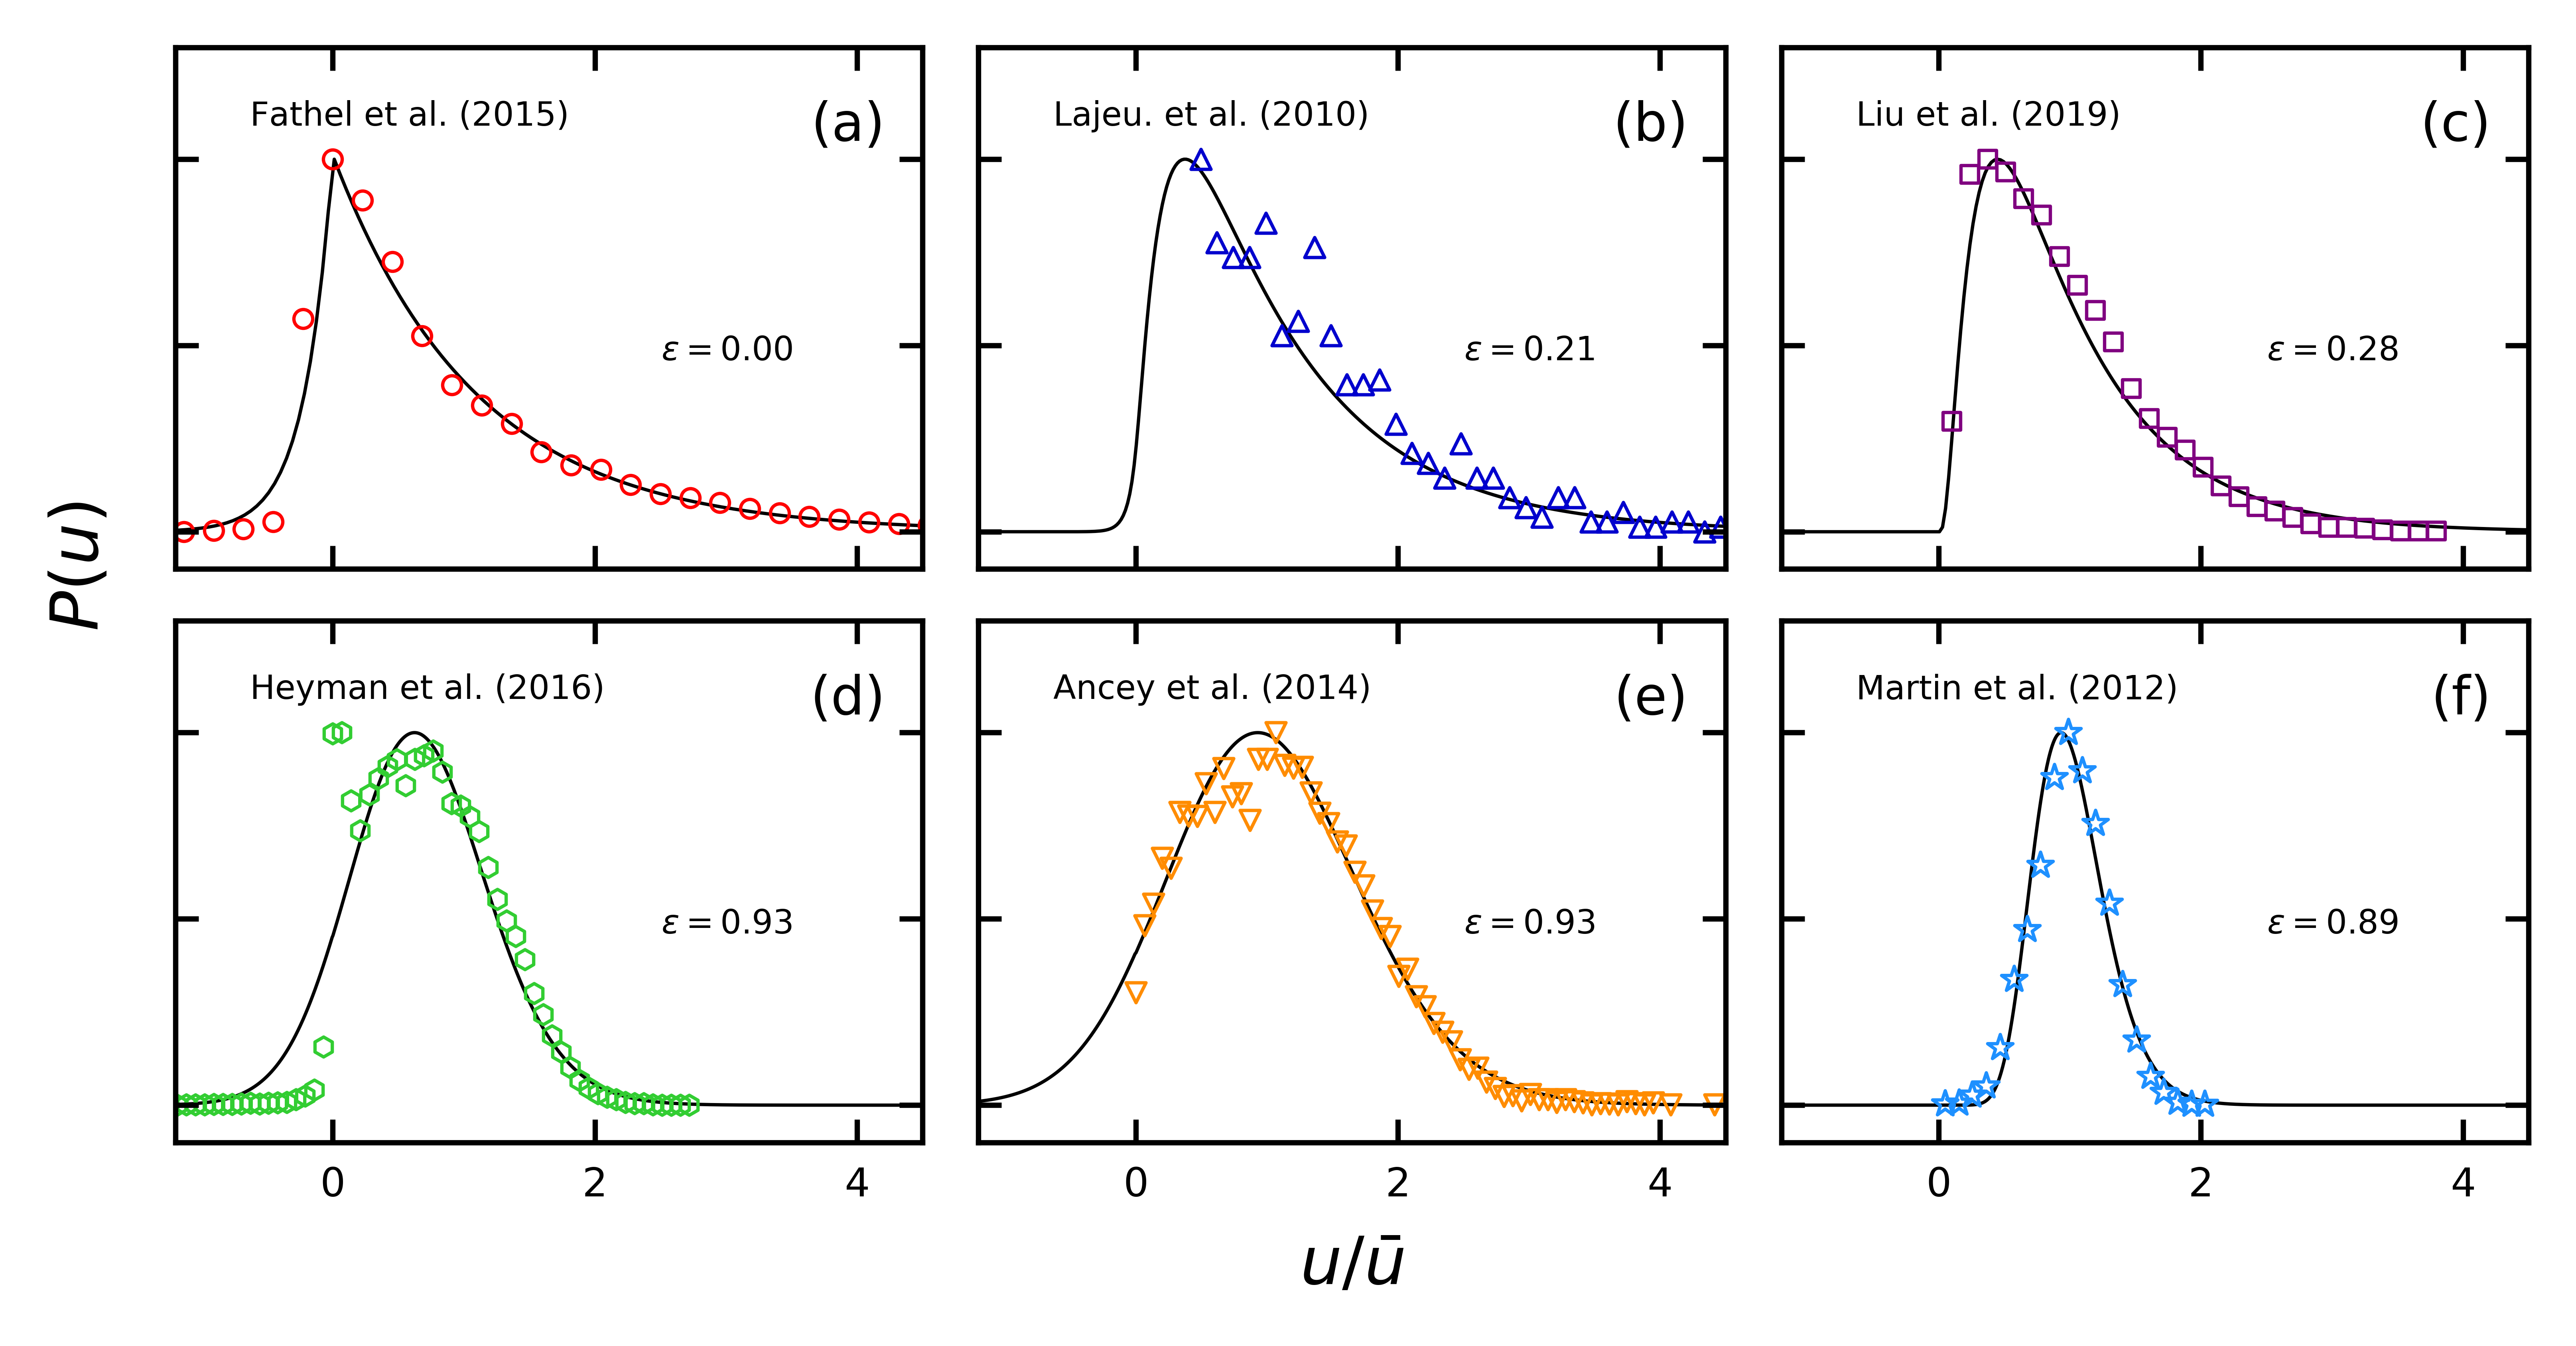
\includegraphics{./figures/ch5/Fig4expComparison.png}}
	\caption{\DIFdelbeginFL \DIFdelFL{This figure compares the }\DIFdelendFL \DIFaddbeginFL \DIFaddFL{The }\DIFaddendFL available experimental data on velocity distributions \DIFdelbeginFL \DIFdelFL{and the theoretical velocity distribution }\DIFdelendFL \DIFaddbeginFL \DIFaddFL{is compared to Eq. }\DIFaddendFL \ref{eq:steadystate} with \DIFaddbeginFL \DIFaddFL{calibration }\DIFaddendFL parameters $\nu$, $\varepsilon$, and $D$\DIFdelbeginFL \DIFdelFL{treated as calibration parameters}\DIFdelendFL . In all cases there is good agreement, indicating that the model \DIFdelbeginFL \DIFdelFL{is capable of }\DIFdelendFL \DIFaddbeginFL \DIFaddFL{produces }\DIFaddendFL the range of distributions \DIFdelbeginFL \DIFdelFL{exhibited by }\DIFdelendFL \DIFaddbeginFL \DIFaddFL{seen in }\DIFaddendFL the experimental data.} \label{fig:fig4ch5}
\end{figure}


\section{Discussion}
\label{sec:langdiscussion}

In this final chapter I developed a Langevin description of \DIFdelbegin \DIFdel{bed load }\DIFdelend \DIFaddbegin \DIFadd{bedload }\DIFaddend sediment transport which includes episodic collisions between particles and the bed.
The model relates the shape of the instantaneous streamwise particle velocity distribution to the elasticity of particle-bed collisions.
This work generalizes earlier approaches available in the literature which did not \DIFdelbegin \DIFdel{treat }\DIFdelend \DIFaddbegin \DIFadd{include }\DIFaddend episodic collisions \citep{Ancey2014,Fan2014}, and provides a new physical explanation for the different streamwise sediment velocity distributions resolved in experiments.

Although in reality, the turbulent forces on moving sediment particles vary in a complex spatio-temporal way, I have approximated the fluid forces on \DIFdelbegin \DIFdel{bed load particles as spatially uniform }\DIFdelend \DIFaddbegin \DIFadd{bedload particles as spatially-uniform }\DIFaddend Gaussian white noise \DIFaddbegin \DIFadd{for reasons of analytical tractability \mbox{%DIFAUXCMD
\cite[e.g.][]{Michaelides1997}}\hspace{0pt}%DIFAUXCMD
}\DIFaddend . Even though the non-Gaussian\DIFaddbegin \DIFadd{, spatiotemporal-varying, }\DIFaddend and history-dependent aspects of fluid turbulence certainly do impact sediment \DIFdelbegin \DIFdel{entrainment }\DIFdelend \DIFaddbegin \DIFadd{movement }\DIFaddend \citep{Cameron2020,Celik2014}, this flow model appears more or less justified since sediment transport experiments provide similar velocity distributions regardless of whether the flow is \DIFdelbegin \DIFdel{viscous }\DIFdelend \DIFaddbegin \DIFadd{laminar }\DIFaddend or turbulent \citep{Lajeunesse2010, Charru2004}, and since particle relaxation times are typically long compared to the timescales of turbulent fluctuations \citep{Hofland2006,Schmeeckle2007,Nakagawa1981}.
\DIFaddbegin \DIFadd{Nevertheless, it is possible the vertical flow structure, and in particular the size of particles in comparison to the thickness of the laminar sub-layer, may be explanatory of the different velocity distributions resolved in bedload transport experiments, and future studies should investigate this possibility.
}\DIFaddend 

The model developed in this chapter described particle-bed collision forces as a sequence of instantaneous impulses in an approach that is reminiscent of the kinetic theory of gases \DIFdelbegin \DIFdel{\mbox{%DIFAUXCMD
\citep{Landau1969}}\hspace{0pt}%DIFAUXCMD
}\DIFdelend \DIFaddbegin \DIFadd{\mbox{%DIFAUXCMD
\citep{Landau1969,Brilliantov2004}}\hspace{0pt}%DIFAUXCMD
}\DIFaddend .
The effect of each collision on the streamwise particle \DIFdelbegin \DIFdel{velocities }\DIFdelend \DIFaddbegin \DIFadd{velocity }\DIFaddend was described by a simple elasticity-like coefficient.
Although such approximate descriptions of particle-particle collisions are common in the theory of granular gases, the elasticity coefficient introduced here is not equivalent to the ``coefficient of restitution" typically applied in granular gas theory.
The coefficient of \DIFdelbegin \DIFdel{resitution }\DIFdelend \DIFaddbegin \DIFadd{restitution }\DIFaddend is defined normal to the contact plane of two particles during a collision, and it characterizes energy loss due to deformation of the colliding particles in the absence of a viscous fluid \citep{Brach1992,Ismail2008}.

In bedload transport, colliding particles are submerged in a viscous fluid, and this introduces additional damping processes besides particle deformation \citep{Joseph2001,Yang2006,Schmeeckle2001}.
The model developed here \DIFdelbegin \DIFdel{did }\DIFdelend \DIFaddbegin \DIFadd{does }\DIFaddend not consider these viscous forces, nor \DIFdelbegin \DIFdel{did }\DIFdelend \DIFaddbegin \DIFadd{does }\DIFaddend it explicitly model the geometry of collisions, as $\ve$ was defined as a parameter applying to the downstream velocity only.
Thus, although I have included episodic particle-bed collisions in a stochastic sediment transport model for the first time, the key parameter \DIFdelbegin \DIFdel{(}\DIFdelend $\ve$ \DIFdelbegin \DIFdel{) }\DIFdelend in this formulation has a rather heuristic character and is not clearly related to the coefficient of restitution from granular gas theory.
Future studies should formulate particle-bed collisions in stochastic sediment transport models considering more details of collision geometry \citep{Sekine1992}, fluid-particle interactions \citep{Marshall2011}, and traditional restitution \citep{Brach1989} using the \DIFaddbegin \DIFadd{stochastic methods in the }\DIFaddend present study as a starting point. 

\subsection{Does the velocity distribution depend on particle size?}

Several researchers have considered why particle velocity distributions differ from one experiment to the next.
One prevailing view is that it relates to flow hydraulics \citep{Wu2020}. Many of the experiments producing Gaussian velocity distributions were conducted in supercritical flows \citep[e.g.][]{Heyman2016,Martin2012,Ancey2014}, whereas many producing exponential distributions were conducted in subcritical flows \citep[e.g.][]{Fathel2015,Charru2004,Seizilles2014}.
However several experiments run counter to this hypothesis.
The experiments of \citet{Lajeunesse2010} produced distinctly exponential velocity distributions in flows well within the supercritical regime ($\Fro=1.5$), whereas \citet{Liu2019} produced Gamma-like distributions in the subcritical regime ($\Fro=0.3$).

An alternative viewpoint, formulated in this chapter, is that the shape of the velocity distribution originates from granular interactions.
Particle size enters the Langevin model \DIFaddbegin \DIFadd{Eq. }\DIFaddend \ref{eq:langevin} explicitly within the steady component of the drag, but it may also enter implicitly through the elasticity parameter $\ve$.
The analytical velocity distribution \DIFaddbegin \DIFadd{Eq. }\DIFaddend \ref{eq:steadystate} was fit to six different experimental datasets in \DIFdelbegin \DIFdel{figure }\DIFdelend \DIFaddbegin \DIFadd{Fig. }\DIFaddend \ref{fig:fig4ch5}, and the best fit parameters \DIFdelbegin \DIFdel{required to for these fits }\DIFdelend were presented in \DIFdelbegin \DIFdel{table }\DIFdelend \DIFaddbegin \DIFadd{Tab. }\DIFaddend \ref{tab:calib}.
These fit parameters suggest collisions are generally less elastic for smaller particle sizes, whereas they are more elastic for larger particle sizes. This suggests that the amount of momentum dissipated by collisions may depend on particle size.

Because the elasticity $\ve$ lumps together collision geometry and dissipation effects, it is challenging to attribute the increasing relationship between elasticity and particle size evident in \DIFdelbegin \DIFdel{table }\DIFdelend \DIFaddbegin \DIFadd{Tab. }\DIFaddend \ref{tab:calib} directly to particle size.
Yet this would be consistent with experiments of idealized particle collisions in viscous fluids. These demonstrate that momentum dissipation varies sharply with particle size, being more elastic for large particles, and less elastic for small particles \citep{Joseph2001,Yang2006,Schmeeckle2001}, exactly like the trend in the table.
A definite conclusion that particle size controls the shape of the bedload velocity distribution requires additional experimental and theoretical study. This \DIFdelbegin \DIFdel{chapter }\DIFdelend \DIFaddbegin \DIFadd{work }\DIFaddend nevertheless produces suggestive ideas.

\section{Summary}
\label{sec:langconclusion}
This chapter has presented a Langevin description of individual bedload particles saltating downstream through episodic collisions.
The model suggests that episodic particle-bed collisions control the shape of the particle velocity distribution, and it is the first model to describe the \DIFdelbegin \DIFdel{full }\DIFdelend range of bedload velocity distributions \DIFdelbegin \DIFdel{that have }\DIFdelend \DIFaddbegin \DIFadd{which have to date }\DIFaddend been reported in experimental studies.

This work \DIFdelbegin \DIFdel{hints that particle size, and not flow hydraulics, may be primarily responsible for }\DIFdelend \DIFaddbegin \DIFadd{suggests that particle-bed collisions be a leading order control over }\DIFaddend the different bedload velocity distributions obtained in experiments, although future study is required for a definite conclusion.
\DIFdelbegin \DIFdel{The next step is }\DIFdelend \DIFaddbegin \DIFadd{Next steps are }\DIFaddend to build up the episodic collision model presented in this chapter to include the geometric details of particle-bed collisions \DIFdelbegin \DIFdel{.
Such an effort }\DIFdelend \DIFaddbegin \DIFadd{and to introduce slip velocity dependence and vertical structure into the flow forces acting on moving particles.
These efforts }\DIFaddend would produce additional insight into the controls of \DIFaddbegin \DIFadd{fluid turbulence and }\DIFaddend transverse, vertical, and rotational movements on the downstream velocities of individual \DIFaddbegin \DIFadd{bedload }\DIFaddend grains.

